%
\RequirePackage{docswitch}
\setjournal{\flag}

\documentclass[\docopts]{\docclass}

% You could define the document class directly
%\documentclass[]{emulateapj}

% 
\usepackage{soul} 
\usepackage{amsmath}
\usepackage{xspace}
\usepackage{xifthen}
\usepackage[dvipsnames,svgnames]{xcolor} 

% General formatting
\newcommand{\ie}{i.e.\xspace}
\newcommand{\eg}{e.g.\xspace}
\newcommand{\etc}{etc.\xspace}
\newcommand{\etal}{et al.\xspace}
\newcommand{\vs}{vs.\xspace}
\newcommand{\super}[1]{\ensuremath{^{\textrm{#1}}}}
\newcommand{\sub}[1]{\ensuremath{_{\textrm{#1}}}}

\newcommand{\FIXME}[1]{{\bf \textcolor{red}{#1}}}
%\newcommand{\FIXME}[1]{{#1}}
\newcommand{\CHECK}[1]{{\bf \textcolor{orange}{#1}}}
%\newcommand{\CHECK}[1]{{#1}}
\newcommand{\COMMENT}[1]{{\it \textcolor{blue}{#1}}}
%\newcommand{\COMMENT}[1]{{#1}}
\newcommand{\NEW}[1]{{\textcolor{blue}{#1}}}
%\newcommand{\NEW}[1]{{#1}}

% Math
\mathchardef\mhyphen="2D
\newcommand{\vect}[1]{\boldsymbol{#1}}
\newcommand{\roughly}{\ensuremath{ {\sim}\,} }
\newcommand{\gtr}{\ensuremath{ {>}\,} }
\newcommand{\less}{\ensuremath{ {<}\,} }
\newlength{\dhatheight}
\newcommand{\doublehat}[1]{%
    \settoheight{\dhatheight}{\ensuremath{\hat{#1}}}%
    \addtolength{\dhatheight}{-0.35ex}%
    \hat{\vphantom{\rule{1pt}{\dhatheight}}%
    \smash{\hat{#1}}}}
\newcommand{\code}[1]{\texttt{#1}\xspace}
\newcommand{\dd}{\ensuremath{\rm d}}
\newcommand{\var}[1]{\ensuremath{#1}\xspace}


% Referencing 
\newcommand{\secref}[1]{Section~\ref{sec:#1}}
\newcommand{\appref}[1]{Appendix~\ref{app:#1}}
\newcommand{\tabref}[1]{Table~\ref{tab:#1}}
\newcommand{\tabrefs}[2]{Tables~\ref{tab:#1} and \ref{tab:#2}}
\newcommand{\figref}[1]{Figure~\ref{fig:#1}}
\newcommand{\figrefs}[2]{Figures~\ref{fig:#1} and \ref{fig:#2}}
\newcommand{\eqnref}[1]{Equation~\eqref{eqn:#1}}

% Astronomy
\newcommand{\LCDM}{\ensuremath{\rm \Lambda CDM}\xspace}
\newcommand{\ra}{{\ensuremath{\alpha_{2000}}}\xspace}
\newcommand{\dec}{{\ensuremath{\delta_{2000}}}\xspace}
\newcommand{\glon}{{\ensuremath{\ell}}\xspace}
\newcommand{\glat}{{\ensuremath{b}}\xspace}

% Units
\newcommand{\unit}[1]{\ensuremath{\mathrm{\,#1}}\xspace}
\newcommand{\Gyr}{\unit{Gyr}}
\newcommand{\MeV}{\unit{MeV}}
\newcommand{\GeV}{\unit{GeV}}
\newcommand{\TeV}{\unit{TeV}}
\newcommand{\degree}{\ensuremath{{}^{\circ}}\xspace}
\newcommand{\mas}{\unit{mas}}
\newcommand{\amin}{\unit{arcmin}}
\newcommand{\asec}{\unit{arcsec}}
\newcommand{\angstrom}{\unit{\AA}}
\newcommand{\um}{\unit{$\mu$m}}
\newcommand{\cm}{\unit{cm}}
\newcommand{\km}{\unit{km}}
\newcommand{\pc}{\unit{pc}}
\newcommand{\kpc}{\unit{kpc}}
\newcommand{\second}{\unit{s}}
\newcommand{\us}{\unit{$\mu$s}}
\newcommand{\photons}{\unit{ph}}
\newcommand{\photon}{\unit{ph}}
\newcommand{\sr}{\unit{sr}}
\newcommand{\Msolar}{\ensuremath{M_\odot}}
\newcommand{\Msun}{\ensuremath{M_\odot}}
\newcommand{\Mstar}{\ensuremath{M_{*}}}
\newcommand{\Lsolar}{\ensuremath{L_\odot}}
\newcommand{\Lsun}{\ensuremath{L_\odot}}
\newcommand{\Lstar}{\ensuremath{L_{*}}}
\newcommand{\Lum}{\ensuremath{ L }\xspace}
\newcommand{\cmcubes}{\ensuremath{\cm^{3}\second^{-1}}\xspace}
\newcommand{\magn}{\unit{mag}}
\newcommand{\mmag}{\unit{mmag}}
\providecommand{\deg}{}
\renewcommand{\deg}{\unit{deg}}
\newcommand{\kms}{{\km\second^{-1}}}
% 


\usepackage[outdir=./]{epstopdf}
\usepackage{graphicx,verbatim}
\usepackage{xspace}

\graphicspath{{./}{./figures/}}
\bibliographystyle{apj}
\newcommand{\todo}[1]{\textcolor{magenta}{To do: #1}}
\newcommand{\mrm}[1]{\mathrm{#1}}

\newcommand{\ccl}{{\tt CCL}\xspace}
\newcommand{\CC}{C\nolinebreak\hspace{-.05em}\raisebox{.3ex}{\footnotesize +}\nolinebreak\hspace{-.10em}\raisebox{.3ex}{\footnotesize +}}

%This is a paper and note template for the LSST DESC
%\citep{Overview,ScienceBook,WhitePaper}. Eventually it will be possible to
%switch between various \LaTeX\xspace styles for internal notes and peer
%reviewed journals templates. The base switch is between \code{aastex.cls} and
%\code{revtex.cls}; however, facilities are also provided for
%\code{emulateapj.cls} and \code{mnras.cls}.\footnote{The \code{mnras.cls} class
%file is a bit odd...} Documents can be compiled using the provided
%\code{Makefile} with several options: \code{make apj}, \code{make apjl},
%\code{make prd}, and \code{make mnras}. There are some oddities when changing
%between templates, so please be patient while we try to work these out.

%There are a number of useful \LaTeX\xspace commands predefined in
%\code{macros.tex}. Notice that the section labels are prefixed with \code{sec:}
%to allow the use of the \verb=\secref= command to reference a section (\ie,
%\secref{intro}). Figures can be referenced with the \verb=\figref= command,
%which assumes that the figure label is prefixed with \code{fig:}. In
%\figref{example} we show an example figure. You'll notice that the actual
%figure file is found in the \code{figures} directory. However, because we have
%specified this directory in our \verb=\graphicspath= we do not need to
%explicitly specify the path to the image.

%The \code{macros.tex} package also contains some conventional scientific units
%like \angstrom, \GeV, \Msun, etc. and some editorial tools for highlighting
%\FIXME{issues}, \CHECK{text to be checked}, \COMMENT{comments}, and \NEW{new
%additions}.

%%%%%%%%%%%%%%%%%%%%%%%%
%% Start the Document %%
%%%%%%%%%%%%%%%%%%%%%%%%

\begin{document}

\title{Core Cosmology Library: Precision Cosmological Predictions for LSST}

\maketitlepre

\begin{abstract}

The Core Cosmology Library (\ccl) provides routines to compute basic
cosmological observables with validated numerical accuracy. These routines have
been validated to an accuracy level, documented here, against the results of
independent implementations. In the current version, predictions are provided
for distances and background quantities, angular auto- and cross-spectra of
cosmic shear, galaxy-galaxy lensing, intrinsic alignments and clustering, halo
bias and the halo mass function. \ccl uses different schemes to obtain the
matter power spectrum, including analytical, phenomenological and other schemes
calibrated through simulations. \ccl is written in C, with a Python interface.
In this note, we explain the functionality of the \ccl library.

\end{abstract}

% Keywords for paper
%\dockeys{latex: templates, papers: awesome}

\maketitlepost

\newpage
\tableofcontents{}
\newpage

\section{Introduction}
\label{sec:intro}

In preparation for constraining cosmology with the Large Synoptic Survey
Telescope (LSST), it is necessary to be able to produce rigorous theoretical
predictions for the cosmological quantities that will be measured. The Core
Cosmology Library\footnote{\url{https://github.com/LSSTDESC/CCL}} (\ccl) aims to
provide, in one library, a way of making predictions that are validated to a
well-documented numerical accuracy, for the purpose of constraining cosmology
with LSST. By constructing a cosmology library specifically with LSST in mind,
it is possible to ensure that it is flexible, adaptable, and validated for all
cases of interest, as well as user-friendly and appropriate for the needs of all
working groups. This note describes the underlying equations and conventions
of the CCL library \citep[see also the CCL paper,][]{Chisari2019}.
The GitHub repository\footnote{\url{https://github.com/LSSTDESC/CCL}} has
installation and usage instructions.

\section{Functionality}
\label{sec:func}

\subsection{Physical constants}
\label{sec:constants}
We have performed a comparison of the physical constants used in \ccl and
included dependencies and external sources. See Table \ref{tab:constants} for
absolute fractional differences of the constants between these sources. Our
final choice of constants for \ccl mainly relies on CODATA 2014 \citep{CODATA14}
in as much as possible, except for ${\rm M}_\odot$, where we adopt the IAU 2015
value \citep{IAU15}, and for the conversion between parsec and meters, where we
take the PDG 2013\footnote{\url{http://pdg.lbl.gov/2013/}} value. Notice that
NIST\footnote{\url{https://physics.nist.gov/cuu/Constants/index.html}} adopts
the CODATA 2014 values.

Notice there are some inconsistencies with the constants adopted by {\tt CLASS}.
This includes the value of the gravitational constant, the Boltzmann constant,
the Planck constant, the speed of light, and the electron charge. Also, the
value of $\rho_c$ is derived from other constants, while PDG 2013 fixes it to a
given value (this is the reason there is only one entry for that column).

After comparison between the physical constants used in \ccl and those of the
sources mentioned above, we have found better than $0.01\%$ agreement for all
constants of interest except for the gravitational constant and the value of the
solar mass.

\begin{table}
  \centering
  \caption{Absolute fractional differences between different constants as tabulated in the sources listed below. Entries marked with zero indicate that this is the value adopted by \ccl. \label{tab:constants}}
  \begin{tabular}{lccccccccc}
    \hline\hline
    & $G_{Newt}$ & $k_b$ & $\sigma_{SB}$ & $h$ & $c$ & eV & $\rho_c$ & $M_\odot$ & pc \\
    \hline
    PDG 2013 & 3e-05 & 2.1e-07 & 1.1e-06 & 7e-08 & 0.0e+00 & 3.5e-08 & 8.8e-10 & 2.2e-05 & 0.0e+00 \\[3pt]
    NIST & 0.0e+00 & 0.0e+00 & 0.0e+00 & 0.0e+00 & 0.0e+00 & 0.0e+00 & \--- & \--- & \--- \\[3pt]
    GSL 2.4 & 1.6e-04 & 1.1e-06 & 5.8e-06 & 6e-09 & 1.5e-06 & 2.1e-06 & \--- & 2.2e-04 & 7.8e-07 \\[3pt]
    CLASS & 3.0e-05 & 1.4e-06 & \--- & 1.6e-07 & 0.0e+00 & 8.4e-08 & \--- & \--- & 1.2e-09 \\[3pt]
    CODATA 2014 & 0.0e+00 & 0.0e+00 & 0.0e+00 & 0.0e+00 & 0.0e+00 & 0.0e+00 & \--- & \--- & \--- \\[3pt]
    IAU 2015 & 0.0e+00 & \--- & \--- & \--- & \--- & \--- & \--- & 0.0e+00 & \--- \\
    \hline\hline
  \end{tabular}
\end{table}




\subsection{Supported cosmological models}
\label{sec:cosmologies}

Ultimately, \ccl plans to incorporate theoretical predictions for all
cosmological models of interest to LSST. Currently, the following families of
models are supported:
\begin{itemize}
    \item Flat $\Lambda$CDM
    \item wCDM and the CPL model ($w_0+w_a$, \citealt{Chevallier01} and \citealt{Linder03})
    \item Non-zero curvature ($K$)
    \item All of the above, plus an arbitrary, user-defined modified growth function (see description in Section \ref{sec:growth})
    \item Massive neutrinos, in combination with any of the above.
    \item $\mu-\Sigma$ modified gravity in combination with the models above
\end{itemize}

\ccl also provides support for modeling the impact of baryons on the matter
power spectrum, as described in Sec. \ref{ss:baryons}. Not all features of \ccl
are available for all models. For a guide to which predictions are available for
each model, see Table \ref{tab:cosmo}. Note that if users install their own
version of {\tt CLASS}, {\tt CCL} can then make predictions for a more extended
set of cosmologies. Users should take care to understand the validity of the
{\tt CCL} assumptions for their own models.

\begin{table*}
  \begin{center}
    \caption{Cosmologies implemented in CCL. \label{tab:cosmo}}
    \begin{tabular}{lccccccc}
      \hline\hline
      Observable/Model & flat $\Lambda$CDM & $\Lambda$CDM+$K$ & $\Lambda$CDM + $m_\nu$ & $w$CDM & $w_0+w_a$    & MG \\[3pt] 
      \hline
      Distances & \checkmark & \checkmark  & \checkmark & \checkmark & \checkmark & $X$ \\
      Growth  & \checkmark & \checkmark & $X$ & \checkmark & \checkmark & \checkmark  \\
      $P_m(k,z)$ & \checkmark & \checkmark & \checkmark & \checkmark & \checkmark & $X$\\
      Halo Mass Function & \checkmark & \checkmark & $X$ & \checkmark & \checkmark & $X$\\
      $C_l$, number counts & \checkmark & $X$ & $X$ & \checkmark & \checkmark & $X$ \\
      $C_l$, weak lensing only & \checkmark & $X$ & \checkmark & \checkmark & \checkmark & $X$ \\
      Correlation function & \checkmark & $X$ & \checkmark & \checkmark & \checkmark & $X$ \\
      \hline\hline
    \end{tabular}
  \end{center}
  %\caption{Cosmologies supported.}
\end{table*}


\subsection{Model Parameterization}

\ccl uses the following cosmological parameters

\begin{description}
  \item[$\Omega_c$] cold dark matter (CDM) density fraction at z = 0
  \item[$\Omega_b$] baryonic matter density fraction
  \item[$h$] Hubble constant in units of 100 {\tt km/s/Mpc}
  \item[$n_s$] primordial scalar perturbation spectral index
  \item[$\Omega_k$] curvature density fraction at z = 0
  \item[$\Omega_g$] radiation density fraction excluding massless neutrinos
  \item[$N_{\rm eff}$] effective number of massless neutrinos
  \item[$m_\nu$] mass or masses of the neutrinos in {\tt eV}
  \item[$w_0$] dark energy equation of state
  \item[$w_a$] amplitude of scale-factor dependence of the dark energy equation of state
  \item[$\mu_0$] one of the $\mu-\Sigma$ modified gravity model parameters
  \item[$\Sigma_0$] one of the $\mu-\Sigma$ modified gravity model parameters
  \item[$A_s$ or $\sigma_8$] amplitude of the matter power spectrum specified either
  primordially ($A_s$) or today ($\sigma_8$)
\end{description}

The parameters $\mu_0$ and $\Sigma_0$ govern the amplitude of modifications to
the cosmological Poisson equation for massive and massless particles respectively
(see sections \ref{sec:growth} and \ref{sec:cl} below for more details). We
currently assume the functional forms \citep{Ferreira2010}
\begin{equation}
\mu(z) = \mu_0 \frac{\Omega_\Lambda(z)}{\Omega_\Lambda(z=0)}\, , \,\,\,
\Sigma(z) = \Sigma_0 \frac{\Omega_\Lambda(z)}{\Omega_\Lambda(z=0)}\ .
\label{muSigform}
\end{equation}

\subsubsection{Specifying Massive and Massless Neutrinos}

\ccl uses either the sum of neutrino masses or a list of values for each in order
to parameterize massive neutrinos. In the case that a sum is provided, \ccl can
use a variety of rules to compute the masses (e.g., normal hierarchy,
inverted hierarchy, or equally split). In the case of the normal or inverted
hierarchy, we use constraints on the squared mass differences from parricle physics
to compute the masses (see \citealt{Lesgourgues2012, Gerbino2017}).

Once all three masses have been specified, we check for which of the three masses
the corresponding neutrino species is non-relativistic today ($m_\nu>0.00017$,
\citealt{Lesgourgues2012}), and thus obtain a number of massive neutrinos
{\tt N$\_$nu$\_$mass}. We use this number along with the {\tt N$\_$eff} value to
set the number of relativistic neutrinos species {\tt N$\_$nu$\_$rel} as follows.
We follow {\tt CLASS} and modify the relationship between the temperature of the
CMB and the neutrino temperature:
\begin{equation}
T_{\nu}^{\rm eff} = T_{\rm CMB} T_{\rm NCDM}
\label{Tnueff}
\end{equation}
where the above defines $T_{\rm NCDM}$, an adhoc modification to the equality
between $T_{\rm CMB}$ and $T_{\nu}^{\rm eff}$. We follow the nomenclature of
{\tt CLASS} here, but we emphasize that $T_{\rm NCDM}$ is a dimensionless
scaling factor, not a temperature. Setting $T_{\rm NCDM}=0.71611$ ensures that
$m_{\nu} / \Omega_{\nu}^0 = 93.14 {\rm eV}$, in agreement with second-order
theoretical calculations which correctly take into account QED effects and
electron / positron annihilation (\citealt{Mangano2005}). Therefore to get
{\tt N$\_$nu$\_$rel} consistent with the {\tt N$\_$eff} passed by the user, we compute:
\begin{equation}
{\tt N\_nu\_rel} = {\tt N\_eff} - \left(T_{\rm NCDM}\right)^{4} \left(\frac{4}{11}\right)^{-\frac{4}{3}} {\tt N\_nu\_mass}.
\label{Nnurel}
\end{equation}

It may sometimes be preferable or necessarily to specify a cosmology in terms
of $\Omega_\nu^0$ for massive neutrinos instead of $m_\nu$. To facilitate this,
\ccl includes a convenience function which takes as input $\Omega_\nu^0$ for
massive neutrinos, the temperature of the CMB, and a label specifying how the
neutrino mass should be split amongst species similarly to above. It then
outputs a pointer to the resulting neutrino mass(es).

\subsection{Distances}
\label{sec:distances}

The Hubble parameter is calculated as
%
\begin{align}\label{eq:Ha}
\frac{H(a)}{H_0} &= a^{-3/2}\Big(\Omega_{M,0}+\Omega_{\Lambda,0} a^{-3(w_0+w_a)}
    \exp[3 w_a (a-1)]+\Omega_{K,0} a \nonumber \\
    &+(\Omega_{g,0} + \Omega_{\nu, {\rm rel}}) a^{-1} + \Omega_{\nu, {\rm m}}(a)a^3\Big)^{\frac{1}{2}}.
\end{align}

The radial comoving distance is calculated via a numerical integral,

\begin{equation}
 \chi(a)= c \int_a^1 \frac{da'}{a'^2 H(a')}.
\end{equation}

The transverse comoving distance is computed in terms of the radial comoving distance as:

\begin{equation}\label{eq:angdist}
 r(\chi)=\left\{\begin{array}{cc}
                 k^{-1/2}\sin(k^{1/2}\chi) & k>0\\
                 \chi & k=0\\
                 |k|^{-1/2}\sinh(|k|^{1/2}\chi) & k<0\\
                \end{array}\right.
\end{equation}

The angular diameter distance between two scale factors is
$d_A(a_1,a_2)=a_2\,r[\chi(a_2)-\chi(a_1)]$ where $a_1>a_2$, and the luminosity distance is
$d_L=r(a)/a$.

\ccl can also compute the distance modulus, defined as,

\begin{equation}\label{eq:distmod}
    \mu = 5 \log_{10}(d_L / {\rm pc})-5\ .
\end{equation}

\subsection{Density parameter functions}
\label{subsec:densityparam}

The density parameter functions $\Omega_X(a)$ can be calculated for six components:
\begin{itemize}
\item matter density parameter $\Omega_M(a) = \Omega_{M,0} H_0^2 / (a^3 H^2(a) )$,
\item dark energy density parameter $\Omega_\Lambda(a) = \Omega_{\Lambda,0} a^{-3(1+w_0+w_a)} \exp[3 w_a (a-1)] H_0^2 / H^2(a)$,
\item radiation density parameter $\Omega_g(a) = \Omega_{g,0} H_0^2 / (a^4 H^2(a) )$,
\item curvature density parameter $\Omega_K(a) = \Omega_{K,0} H_0^2 / (a^2 H^2(a) )$,
\item massless neutrino density parameter $\Omega_{\nu, {\rm rel}}(a) = \Omega_{\nu, {\rm rel},0} H_0^2 / (a^4 H^2(a) )$,
\item massive neutrino density parameter $\Omega_{\nu, {\rm m}}(a)$,
\end{itemize}
all using the Hubble parameter defined in equation~\ref{eq:Ha}.

For massive neutrinos, $\Omega_{\nu, {\rm m}}(a)$ is calculated as follows.
For each species of massive neutrino with mass $m_\nu^i$, we define

\begin{equation}
\tilde{m}^i = \frac{m_{\nu}^{i}a}{T_{\nu}^{\rm eff}}
\label{mnuOT}
\end{equation}
in units such that $\tilde{m}$ is dimensionless. We then multiply by the appropriate
factors to obtain $\Omega_{\nu, {\rm m}}(a)$:

\begin{equation}
\Omega_{\nu, {\rm m}}(a) = \sum_{i=1}^{N_\nu} \frac{8 \pi^2(\pi k_b )^3 k_b}{15(c h_{\rm P})^3} \frac{8 \pi G}{3h^2c^2}
\left(\frac{T_{\nu}^{\rm eff}}{a}\right)^4 \left(\frac{7}{8}\int_0^{x_{\rm max}} dx \, x^2
\frac{\sqrt{x^2 + \left(\tilde{m}^i\right)^2}}{\exp(x) + 1}\right)
\label{Omnu}
\end{equation}
where $h_{\rm P}$ is Planck's constant and $h$ is $H_0/100$ with $H_0$ in units
of {\tt km / s / Mpc}. $x_{\rm max}$ is set to 1000. The final bracketed term
which includes the phase-space integral can be simplified in the limit where
$\tilde{m}$ is very large or very small: for small $\tilde{m}$, it is set to
$\frac{7}{8}$, and for large $\tilde{m}$, it becomes
$\frac{5\zeta(3)}{18\pi^4}\tilde{m}\sim 0.2776\mu$.

\subsection{Functions of the physical density}
\label{subsec:physicaldensity}

The physical density $\rho_X(a)$ can be calculated for seven components:
\begin{itemize}
\item critical density $\rho_{\rm crit}(a) = {{3 H^2(a)} \over { 8 \pi G}} = \rho_{\rm crit,0} H^2(a) / H_0^2$,
\item matter density $\rho_M(a) = \rho_{\rm crit}(a) \Omega_M(a) = \rho_{\rm crit,0} \Omega_{M,0} / a^{3}$,
\item dark energy density parameter $\rho_\Lambda(a) = \rho_{\rm crit,0} \Omega_{\Lambda,0} a^{-3(1+w_0+w_a)} \exp[3 w_a (a-1)]$,
\item radiation density parameter $\rho_g(a) = \rho_{\rm crit,0} \Omega_{g,0} / a^{4}$,
\item curvature density parameter $\rho_K(a) = \rho_{\rm crit,0} \Omega_{K,0} / a^{2}$,
\item massless neutrino density parameter $\rho_{\nu, {\rm rel}}(a) = \rho_{\rm crit,0} \Omega_{\nu, {\rm rel},0} / a^{4}$,
\item massive neutrino density parameter $\Omega_{\nu, {\rm m}}(a) = \rho_{\rm crit,0} \Omega_{\nu, {\rm m}}(a) H^2(a) / H_0^2$,
\end{itemize}
where $\Omega_{\nu, {\rm m}}(a)$ is given by equation~\ref{Omnu} and the Hubble
parameter by equation~\ref{eq:Ha}. \ccl moreover allows for comoving physical
densities $\rho_{X, {\rm comoving}}(a) = \rho_X(a) a^3$.


\subsection{Growth function}
\label{sec:growth}

To compute $D(a)$, the growth factor of matter perturbations, \ccl solves the
following differential equation:
\begin{equation}
  \frac{d}{da}\left(a^3H(a)\frac{dD}{da}\right)=\frac{3}{2}\Omega_M(a)aH(a)D,
\end{equation}
using a Runge-Kutta Cash-Karp algorithm.

In doing this, \ccl simultaneously computes the growth rate $f(a)$, defined as:
\begin{equation}
  f(a)=\frac{d\ln D}{d\ln a}.
\end{equation}
\ccl provides different functions that return the growth
normalized to $D(a=1)=1$ and to $D(a\ll1)\rightarrow a$.

Note that the above is strictly valid for a Universe containing only dust-like
matter components. A scale-independent growth rate is, for example, ill-defined
in the presence of massive neutrinos; therefore \ccl will raise an error if the
user attempts to calculate the growth rate or growth factor in a cosmology
with massive neutrinos.

Currently, \ccl allows for two version of alternative `modified gravity'
cosmological models. The first is defined by a regular background
$(w_0+w_a)$CDM (with arbitrary $K$) as well as a user-defined $\Delta f(a)$,
such that the true growth rate in this model is given by $f(a)=f_0(a)+\Delta f(a)$,
where $f_0(a)$ is the growth rate in the background model. Note that this
implementation of `modified gravity' is only consistently implemented with
regards to the computation of the linear growth factor and growth rates
(which will also scale the linear power spectrum). All other \ccl functions
(including the non-linear power spectrum) will ignore these modifications.
This model, and the interpretation of the predictions given by \ccl,
should therefore be used with care.

The second model for deviations from General Relativity supported by \ccl is
the quasistatic parameterization, with parameterizing functions $\mu(a)$ (
the change to the Poisson equation for massive particles) and $\Sigma(a)$ (
the change to the same for massless particles), with functional form assumed to
be given as in equation \ref{muSigform}. The background is once again allowed
to be defined by $(w_0+w_a)$CDM (with arbitrary $K$).

The growth factor and growth rate are altered when ${\tt mu\_0} \ne 0$, with
the above equation becoming
\begin{equation}
  \frac{d}{da}\left(a^3H(a)\frac{dD}{da}\right)=\frac{3}{2}\Omega_M(a)aH(a)(1 + \mu(a))D.
\end{equation}
As usual, the resulting growth factor can be returned normalized to
$D(a=1)=1$ or to $D(a\ll1)\rightarrow a$. The second normalization is used in
returning the matter power spectrum with appropriate modification in this model,
as discussed in section \ref{sec:power}.

\subsection{Matter power spectrum}
\label{sec:power}

There are several options for obtaining the linear and non-linear matter power
spectrum in \ccl. We parameterize the linear matter power spectrum via the
transfer function via the relationship $P(k) = 2 \pi^2 \Delta^2(k) /k^3  \propto
T^2(k) k^{n_s}$, where $\Delta(k)$ is the dimensionless power spectrum and $n_s$
is the spectral index. The normalization of the power spectrum is defined at
$z=0$ by setting $\sigma_8$ to its value today or by setting the initial value
$A_s$. The non-linear matter power spectrum options either use the linear
matter power spectrum as inputs (e.g., the halo model) or supply their own
values (e.g., an emulator). Both power spectra are interpolated
in a two-dimensional table of scale factor and redshift for later use.

\subsubsection{BBKS}
\ccl implements the analytical BBKS approximation to the transfer function \citep{BBKS}, given by
\begin{equation}
T(q\equiv k/\Gamma h {\rm Mpc}^{-1}) = \frac{\ln[1+2.34q]}{2.34q}[1+3.89q+(16.2q)^2+(5.47q)^3+(6.71q)^4]^{-0.25}
\end{equation}
where $\Gamma = \Omega_m h$.

The BBKS power spectrum option is primarily used as a precisely-defined input
for testing the numerical accuracy of \ccl routines. It is not recommended for
other uses as it is only accurate to a few percent.

\subsubsection{Eisenstein and Hu}
\ccl also provides an approximation to the transfer function as implemented by
\citet{1998ApJ...496..605E} (E\&H; we refer the reader to this paper for a detailed
discussion of the fitting formulae).\footnote{
  Note that the implementation in \ccl is different from that in \citet{1998ApJ...496..605E}
  in two places. First, \ccl modifies Eq. 5 of \citet{1998ApJ...496..605E} using
  $a^{-1}=1+z$ instead of the approximation $a^{-1}\sim z$. The difference
  in the resulting power spectra is negligible, but larger than 1 part
  in $10^4$ for $k<10\,h\,{\rm Mpc}^{-1}$. Second, \ccl modifies the argument of
  $G$ in Eq. 14 to be $zeq/(1+zd)$ instead of $(1+zeq)/(1+zd)$.}

The Eisenstein \& Hu approximation is also not very accurate (generally only
to within a few percent), and so should not be used to derive
precise cosmological constraints.

\subsubsection{CLASS}
\ccl can call the {\tt CLASS} software package \citep{class}
to obtain the linear matter power spectrum at given redshift. On
initializing the cosmology object, we construct a bi-dimensional spline in $k$
and the scale-factor which is then evaluated by the relevant routines to obtain
the matter power spectrum at the desired wavenumber and redshift.

\subsubsection{CAMB}
The fiducial configuration calls the {\tt CAMB} package \citep{camb}
to obtain the linear matter power spectrum at given redshift. On
initializing the cosmology object, we construct a bi-dimensional spline in $k$
and the scale-factor which is then evaluated by the relevant routines to obtain
the matter power spectrum at the desired wavenumber and redshift.

\newpage

\subsubsection{ISiTGR}
\ccl can call the {\tt ISiTGR} software patch \citep{isitgr1,isitgr2} that is 
built on the top of the {\tt CAMB} package to include modified gravity models. 
This is invoked by specifying the transfer function option boltzmann\_isitgr. 
\ccl then then calculates the GR or modified gravity linear matter power spectrum 
at a given redshift. Here also, on initializing the cosmology object, we construct a 
bi-dimensional spline in $k$ and the scale-factor which is then evaluated by the 
relevant routines to obtain the matter power spectrum at the desired wavenumber 
and redshift.

\subsubsection{Halofit}
We provide a Halofit implementation that applies a correction to any input
linear matter power spectrum to compute an approximation to the non-linear
matter power spectrum. We use the model from \citet{CLASS_halofit} which is
accurrate to roughly $10\%$.

\subsubsection{Halo Model}
We also provide a halo model implementation for computing the non-linear matter
power spectrum. Halo model computations are known to be inaccurate at the $10\%$
level or more. See Section~\ref{sec:halo_model} for details.

\subsubsection{Nonlinear Perturbation Theory}
We provide an implementation of nonlinear standard perturbation theory (SPT) for the matter power spectrum
using the {\tt FAST-PT} package \citep{mcewen16}. SPT provides a reasonable approximation of the matter
power spectrum in the mildly nonlinear regime but breaks down on smaller scales.
It is also known to provide a poor correction to the BAO feature.
This perturbation theory implementation is discussion in more detail in Section~\ref{sec:Nonlinear_Pk}.

\subsubsection{Cosmic emulator}

The cosmic emulator of \citet{Lawrence17} is integrated into \ccl and it is
available as one of the non-linear matter power spectrum options. The cosmic
emulator provides predictions for the non-linear matter power spectrum based on
an interpolation over simulation outputs spanning a defined set of cosmological
parameter values.

The emulator provides accurate predictions for the nonlinear matter power
spectrum, at the $1\%$ level, for $z\leq 2$ and in the wavenumber range
$k=[10^{-3},5]$ Mpc$^{-1}$. If a redshift above $z=2$ is passed, the emulator
will quit and return an error message. For $k$ values below and above the
previously specified range, we extrapolate in the manner specified in the
following section.

The allowed range of cosmological parameters is as follows:
\begin{eqnarray}
0.12&\leq& \Omega_m h^2 \leq 0.155,\nonumber\\
0.0215&\leq& \Omega_b h^2 \leq 0.0235,\nonumber\\
0.7&\leq& \sigma_8 \leq 0.9,\nonumber\\
0.55&\leq& h \leq 0.85,\nonumber\\
0.85&\leq& n_s\leq 1.05,\nonumber\\
-1.3&\leq& w_0\leq-0.7,\nonumber\\
-1.73&\leq& w_a\leq -0.7,\nonumber\\
0.0&\leq& \Omega_\nu h^2 \leq 0.01.
\end{eqnarray}
 %
Further, $w_a$ and $w_0$ are constrained jointly to be $0.3\leq (-w_0-w_a)^{1/4}$.
Note that \ccl only allows a subregion within this parameter space. For models in which w(z) crosses $-1$ at some
given redshift, {\tt CLASS} will crash because this value corresponds
to a true cosmological constant, which by definition should have no
perturbations.\footnote{
  We thank Emilio Bellini and Miguel Zumalac\'arregui for clarifying this for us.}

\paragraph{Neutrino species} The emulator is set up to consider $N_{\rm eff}=3.04$
and to allow the user to provide $\Omega_\nu h^2$ in order to set the
neutrino mass, where it is assumed that the corresponding mass is split equally
amongst three neutrinos. This is different from the standard {\tt CCL}
configuration, which takes as input the mass(es) of neutrinos in eV, $m_{\nu}$.
The assumption of an equal split of masses amongst three neutrino species is
also different from the default \ccl choice to split the mass amongst species
according to the normal hierarchy. We allow models with non-equal masses to use
the emulator by calling it with the total mass in neutrinos split equally between
the different species. This choice may result in internal inconsistency amongst
different quantities calculated with the same \ccl cosmology, or indeed even
internal inconsistency between the linear and nonlinear parts of the same
power spectrum. Note also that because the emulator is constructed with
$N_{\rm eff}=3.04$, the user is required to pass this value when the emulator
is in use.

Notice that ideally we would like to pass a non-integer number of massive
neutrino species for best compatibility with the emulator set-up. However,
since this is not possible within {\tt CCL}, we have opted to verify that neither
the growth function nor the comoving radial distance computation are affected by
this approximation to more than $10^{-4}$ in the range $0.01<a<1$, where $a$ is
the scale factor. We have verified this by comparing this prediction for a
fiducial cosmology $\{\Omega_c=0.27,\Omega_b=0.049,h=0.67,\sigma_8=0.8,n_s=0.96\}$
with the following neutrino parameters:
$\{N_{\nu,{\rm rel}},N_{\nu,{\rm mass}},m_{\nu}\}=\{0.00641,3,0.06{\rm eV}\}$, $\{N_{\nu,{\rm rel}},N_{\nu,{\rm mass}},m_{\nu}\}=\{0,3.04,0.06{\rm eV}\}$ and
$\{N_{\nu,{\rm rel}},N_{\nu,{\rm mass}},m_{\nu}\}=\{0,3.046,0.06{\rm eV}\}$. The
discrepancy between distances and growth results between these choices of
neutrino parameters can raise above $10^{-4}$ at $a<0.01$ and the user should
be mindful of this for their particular application.

\subsubsection{Impact of baryons}
\label{ss:baryons}

\ccl incorporates the impact of baryons on the total matter power spectrum via
the ``baryonic correction model'' (BCM) of \citet{Schneider15}. When this
correction is in use, the nonlinear matter power spectrum (whichever the
method that provides it) is multiplied by a correction factor $F(k,z)$ which
models the impact of baryons.

The main consequences of baryonic processes are: to suppress the power spectrum
at intermediate scales ($k\sim$ a few $h/$Mpc) due to the ejection of gas by
Active Galactic Nuclei feedback, and to enhance it at smaller scales due to
enhanced cooling. Three effective parameters govern the contribution of baryonic
processes to modifying the total matter power spectrum:

\begin{itemize}
  \item $\log_{10} [M_c/($M$_\odot/h)]$: the mass of the clusters responsible for
    feedback, which regulates the amount of suppression of the matter power spectrum at intermediate scales
  \item $\eta_b$: a dimensionless parameter which determines the scale at which suppression peaks
  \item and $k_s$ [$h/$Mpc]: the wavenumber that determines the scale of the stellar profile
\end{itemize}

If the BCM parameters are not specified and the user sets \ccl to compute the power
spectrum with baryonic feedback included, \ccl will assume the default parameters
of \citet{Schneider15}.

\subsubsection{Modified gravity ($\mu, \Sigma$)}

\ccl supports the quasistatic parameterization of modified gravity with
scale-independent deviations from GR which arise at late times (currently with
functional form given in equation \ref{muSigform}). Under these conditions,
and the specified cosmology, the modified gravity matter power spectrum is
calculated using {\tt ISiTGR}  (described further above) according to the values of the modified 
gravity parameters. If these are zero or not specified then the GR matter power 
spectrum is calculated.

This implementation replaces the intilal one where the modified gravity power 
spectrum is computed by re-scaling the GR matter power spectrum by 
multiplying it by the squared ratio of the MG  growth factor $D_{MG}$ to the GR 
one, $D_{GR}$. 

The new implementation solved accuracy issues for spectra and  correlations 
encoutered in the initial implementation and provides the power  spectrum and 
the 2D angular spectra and correlations at the same level of accuracy 
as that of the LCDM standard model.   

The splines for the power spectrum are then set as usual, but we note that 
the $\mu, \Sigma$ MG implementation is valid only in the quasistatic limit 
and is also restricted to the linear regime for now since no-reliable methods 
are available to model such non-linear small scales nor the very 
large scales where the quasistatic limit cease to be valid.   

\subsubsection{Extrapolation for the nonlinear power spectrum}
\label{sec:NLextrapol}

The computation of the power spectrum from {\tt CLASS} can be significantly sped
up by extrapolating in the range $k>$~{\tt K$\_$MAX$\_$SPLINE} and
$k<$~{\tt K$\_$MIN$\_$SPLINE}. In this section, we describe the implementation of the
extrapolation and the accuracy attained. These tests are performed in a flat
$\Lambda$CDM cosmology with $\Omega_c=0.25$, $\Omega_b=0.05$,
$A_s=2.1\times10^{-9}$, $h=0.7$ and $n_s=0.96$.

We first describe the extrapolation at high wavenumbers. The introduction of
the parameter {\tt K$\_$MAX$\_$SPLINE} allows us to spline the matter power
spectrum up to that value of $k$ (in units of $1/$Mpc). A separate {\tt K$\_$MAX}
parameter sets the limit for evaluation of the matter power spectrum. The range
between {\tt K$\_$MAX$\_$SPLINE}$<k<${\tt K$\_$MAX} is evaluated by performing
a second order Taylor expansion in $\ln k$.

First, we compute the first and second derivative of the $\ln P(k,z)$ at
$k_0={\rm \tt K\_MAX\_SPLINE}-2\Delta\ln k$ by computing the numerical
derivatives by finite differences using {\tt GSL}. The fiducial choice for
$\Delta\ln k$ is $10^{-2}$. We then apply a second order Taylor expansion to
extrapolate the matter power spectrum to $k>${\tt K$\_$MAX$\_$SPLINE}.
The Taylor expansion gives
%
\begin{equation}
  \ln P(k,z) \simeq \ln P(k_0,z) + \frac{d\ln P}{d\ln k}(\ln k_0,z) (\ln k-\ln k_0)  + \frac{1}{2}  \frac{d^2\ln P}{d\ln k^2}(\ln k_0,z) (\ln k-\ln k_0)^2.
  \label{eq:NLPSTaylor}
\end{equation}

The accuracy of this approximation is shown in Figure \ref{fig:NLextrapol} for
redshifts $z=0$, $z=3$ and $z=20$. We compare the nonlinear matter power
spectrum at these redshifts, computed with the previously described approximation,
to the matter power spectrum obtained by setting the power spectrum splines to
high values. We find that for typical values of $\Delta \ln k=10^{-2}$ and
{\tt K$\_$MAX$\_$SPLINE}$=50$/Mpc, $\ln P$ has converged to an accuracy that
surpasses the expected impact of baryonic effects on the matter power spectrum
at $k>10/$Mpc. (For an estimate of the impact of baryons on the total matter
power spectrum, see \citealt{Schneider15}.) The lower {\tt K$\_$MAX$\_$SPLINE}
is, the faster \ccl will run. The optimum choice of {\tt K$\_$MAX$\_$SPLINE} is
left to the user for their particular application.

We also extrapolate the power spectrum at small wavenumbers. In this case,
the power spectrum below {\tt K$\_$MIN$\_$SPLINE} is obtained by a power-law
extrapolation with index $n_s$:
\begin{equation}
  \log P(k<{\tt K\_MIN\_SPLINE},z) = \log P({\tt K\_MIN\_SPLINE},z) + n_s (\log k-\log{\tt K\_MIN\_SPLINE})
\end{equation}
The value adopted for {\tt K\_MIN\_SPLINE} depends on the choice of power
spectrum method and is not currently settable by the user. For {\tt CLASS} and
the nonlinear power spectrum, we adopt {\tt K\_MIN\_SPLINE} that coincides with
the smallest wavenumber output by {\tt CLASS}, {\tt K\_MIN\_SPLINE}$=7\times 10^{-6}$/Mpc.
Note that this parameter is different from {\tt K\_MIN}, which sets the minimum
$k$ for integrations and which is set by default to {\tt K\_MIN}$=5\times 10^{-5}$/Mpc.
Hence, in practice, no extrapolation is occurring in this case, unless the user
specifically asks for an output power spectra below {\tt K\_MIN} for their own purposes.

For BBKS, the power spectrum is computed analytically at all $k$, there is no
extrapolation. For the Eisenstein \& Hu implementation, the splines of the power
spectrum span {\tt K\_MIN}$<k<${\tt K$\_$MAX$\_$SPLINE}, so there is only
extrapolation at high $k$. For the nonlinear matter power spectrum from the
emulator, {\tt K\_MIN\_SPLINE} and {\tt K\_MAX\_SPLINE} are set to fixed values
that are determined from the range of validity of the emulator:
{\tt K\_MIN\_SPLINE}$=10^{-3}$ Mpc$^{-1}$ and {\tt K\_MAX\_SPLINE}$=5$ Mpc$^{-1}$.


%------------------------
\begin{figure*}
\centering
  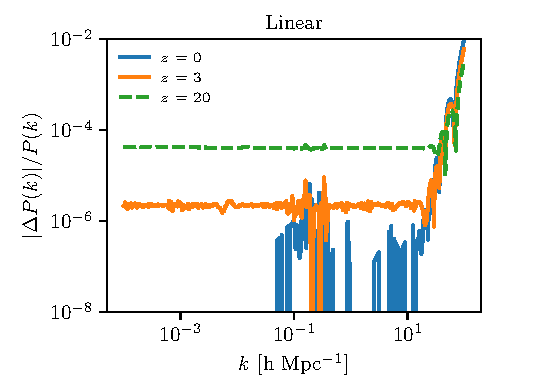
\includegraphics[width=0.49\textwidth]{splacc_power_lin}
  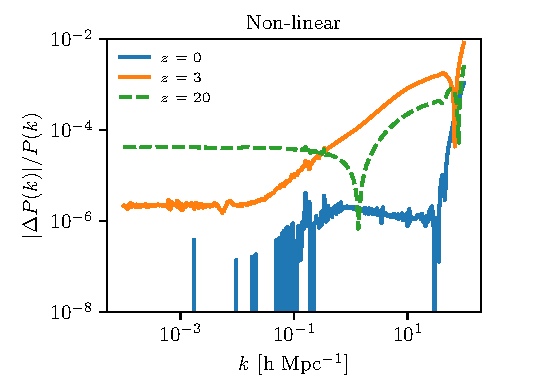
\includegraphics[width=0.49\textwidth]{splacc_power_nl}
\caption{
    The relative error compared to power spectra produced with high values of the
    power spectrum splines, $P_{fid}$, produced by splining the matter power
    spectrum up to {\tt K$\_$MAX$\_$SPLINE}$=50\,\text{Mpc}^{-1}$ and extrapolating
    beyond this value with a second order Taylor expansion the natural logarithm of
    the matter power spectrum. The left panel shows the relative errors for the
    linear matter power spectrum at $z=0$, $z=3$ and $z=20$. The right panel shows
    the results for the non-linear matter power spectrum at the same redshifts. The
    standard \ccl parameters adopted are those corresponding to the black dashed
    curve. For comparison, the impact of baryonic physics on the matter power
    spectrum is $\sim 10\%$ at $k=1\,\text{Mpc}^{-1}$ \citep{Schneider15}.}
\label{fig:NLextrapol}
\end{figure*}
%------------------------

\subsubsection{Extrapolation for the linear power spectrum}
\label{sec:Lextrapol}

With the implementation described in the previous section, the power spectrum
splines are initialized up to {\tt K$\_$MAX$\_$SPLINE}. This is also true for
the linear matter power spectrum, which is used within \ccl in particular to
obtain $\sigma_8$ (see Eq. \ref{eq:sigR}). We have tested here how the procedure
described in the previous section affects the convergence of the linear
matter power spectrum. The result is shown in Figure \ref{fig:NLextrapol}. For
some applications that use the linear power spectrum, the user might need to
increase the value of {\tt K$\_$MAX$\_$SPLINE}.

As in the previous section, the power spectrum at small wavenumber is extrapolated
using a power-law. This extrapolation is performed below a fiducial value of
{\tt K\_MIN\_SPLINE} that coincides with the smallest wavenumber output by
{\tt CLASS}, as in the case of the nonlinear power spectrum described above.

We have found that changing the sampling in scale factor to $200$, or changing
the sampling of the wavenumber to $5000$ points, does not change the results
presented in Figure~\ref{fig:NLextrapol}.


\subsubsection{Normalization of the power spectrum}
\label{sec:PSnorm}

There are two schemes for normalization of the matter power spectrum. The first
one is to specify the value of $A_s$, the amplitude of the primordial power
spectrum, which is passed directly to {\tt CLASS}. Alternatively, there is the
option to set the normalization of the matter power spectrum by specifying
$\sigma_8$, the RMS density contrast averaged over spheres of radius
$8h^{-1}$Mpc. Note that for linear power spectrum models where {\tt CLASS} is not
used, only the option to specify $\sigma_8$ is supported. The computation of
$\sigma_8$ is described in Section \ref{sec:hmf}.

\subsubsection{Non-linear scale cut}
\label{sec:kNL}

The scale at which non-linear structure formation becomes important for the computation of the matter power spectrum at a particular redshift can be estimated using
\begin{equation}
k_NL(z) \approx \Sigma(z)^{-1}=\left[ \frac{1}{6\pi^2} \int^{\infty}_0 dk P_{\rm lin}(k,z) \right]^{-1/2}~.
\end{equation}

\subsection{Nonlinear Power Spectra}
\label{sec:Nonlinear_Pk}

Nonlinear perturbation theory (e.g.\ \citealp{bernardeau02}) provides a method to calculate power spectra in the mildly nonlinear regime. {\tt CCL} provides perturbation theory predictions for dark matter clustering, galaxy biasing, and intrinsic alignments using the {\tt FAST-PT} package \citep{mcewen16,fang17}. These predictions can be used as the general input for the power spectra between observables $\alpha$ and $\beta$, $P_{\alpha\beta}$, as described below in \ref{sec:cl}. Currently, all modeling is done at ``one-loop'' order, i.e.\ $\mathcal{O}(P_{\rm lin}^2)$, in standard perturbation theory (SPT). \ccl implements these models using {\tt PTTracer} objects.

\subsubsection{Matter density}

The matter density field can be expanded:
\begin{equation}
  \label{eq:delta_spt}
  \delta_m = \delta^{(1)} + \delta^{(2)} + \delta^{(3)} + \cdots,
\end{equation}
where $\delta^{(1)}$ is the linear density field and higher-order terms can be expressed as a function of the linear density field at the specified order. The matter power spectrum is then given by:
\begin{equation}
  P_{\rm NL} = P_{11} + P_{22} + 2P_{13}~,
\end{equation}
where $P_{11}$ is $P_{\rm lin}$.

Note that the nonlinear treatments of galaxy bias and intrinsic alignments use the one-loop SPT matter density expression when calculating relevant correlations, even if a different nonlinear prescription is used for $P_{\rm NL}$.

\subsubsection{Galaxy bias}
See \cite{desjacques18rev} for a detailed discussion on galaxy bias and treatments in perturbation theory. Currently, nonlinear galaxy bias is given by the following expression (e.g.\ \citealp{baldauf12}):
\begin{equation}
  \delta_{g} = b_1 \delta_m +\frac{b_2}{2} (\delta_m^2 - \langle \delta_m^2 \rangle) +
  \frac{b_s}{2} (s^2 - \langle s^2 \rangle) ~,
\end{equation}
where $s$ is the tidal field, and the mean values of both quadratic quantities are subtracted.
The standard linear bias is $b_1$, and $(b_2,b_s)$ are the quadratic bias coefficients.
The relevant galaxy-galaxy (for two galaxy samples, denoted by the second superscript) and galaxy-matter power spectra are then:
\begin{align}
  &P_{gg} = b_{1,1} b_{1,2} P_{d1d1} +
               \frac{1}{2} (b_{1,1} b_{2,2} + b_{1,2} b_{2,1}) P_{d1d2} \notag\\
               &~~~~ + \frac{1}{4} b_{2,1} b_{2,2} P_{d2d2} +
               \frac{1}{2} (b_{1,1} b_{s,2} + b_{1,2} b_{s,1}) P_{d1s2} \notag\\
               &~~~~ + \frac{1}{4} (b_{2,1} b_{s,2} + b_{2,2} b_{s,1}) P_{d2s2} +
               \frac{1}{4} b_{s,1} b_{s,2} P_{s2s2}~,\\
  &P_{gm} = b_1 P_{d1d1} + \frac{1}{2}b_2 P_{d1d2} + \frac{1}{2} b_s P_{d1s2}~,
\end{align}
where $P_{d1d1}$ corresponds to the chosen nonlinear matter power spectrum,
and the other terms are one-loop PT expressions.

\subsubsection{Intrinsic alignments}

Following the ``TATT'' model (tidal alignment and tidal torquing) described in \cite{blazek19}, the galaxy intrinsic alignment field can be expanded:
\begin{equation}
    \gamma^{I}_{ij} = C_1 s_{ij} + C_2\left( s_{ik} s_{kj} - \frac{1}{3}\delta_{ij} s^2 \right) + C_{1\delta} (\delta s_{ij})~.
\end{equation}
Higher-order contributions will be included in future releases. The matter-intrinsic and intrinsic-intrinsic ($E$- and $B$-mode) power spectra are given by:
\begin{align}
\label{eq:dEtot}
P_{\delta E} =& C_1 P_{d1d1} + C_{1\delta} \left[A_{0|0E} + C_{0|0E}\right]
+ C_2 \left[ A_{0|E2} + B_{0|E2}\right]~, \\
\label{eq:EEtot}
P_{EE} =&
C_{1,1}C_{1,2} P_{d1d1} + (C_{1,1} C_{1\delta,2}+C_{1,2} C_{1\delta,1}) \left[A_{0|0E}+ C_{0|0E}\right] + C_{1\delta,1} C_{1\delta,2} A_{0E|0E} \notag\\
&+ C_{2,1} C_{2,2} A_{E2|E2} + (C_{1,1} C_{2,2} + C_{1,2} C_{2,1}) \left[ A_{0|E2} + B_{0|E2}\right] \notag \\
&+ (C_{1\delta,1} C_{2,2} + C_{1\delta,2} C_{2,1})D_{0E|E2}~,\\
\label{eq:BBtot}
P_{BB} =& C_{1\delta,1} C_{1\delta,2} A_{0B|0B} + C_{2,1} C_{2,2} A_{B2|B2} + (C_{1\delta,1} C_{2,2} + C_{1\delta,2} C_{2,1}) D_{0B|B2} ~,
\end{align} 
where, as above, $P_{d1d1}$ corresponds to the chosen nonlinear matter power spectrum,
and the other terms are one-loop PT expressions.

The normalization of the IA bias parameters can be flexibly specified. The convention of \cite{blazek19} is
\begin{align}
    C_1(z) = - A_{1}(z) \frac{\bar{C}_1 \Omega_{\rm m} \rho_{\rm crit}}{D(z)}~, \\
    C_{1 \delta}(z) = - A_{1 \delta}(z) \frac{\bar{C}_1 \Omega_{\rm m} \rho_{\rm crit}}{D(z)}~, \\
    C_{2}(z) = A_{2}(z) \frac{5\bar{C}_1 \Omega^2_{\rm m} \rho_{\rm crit}}{\Omega_{\rm m,fid} D^2(z)}~.
\end{align}
This convention for $C_1(z)$ matches the default \ccl normalization for $b_{\rm IA}$ used in the standard WL tracer, in which the user is assumed to be specifying $A_{1}$ (see Eq.~\ref{eq:bIA_norm}). When using this nonlinear TATT model, the full $z$-dependent $C$-values must be specified, and the IA amplitude in the standard WL tracer must be set to one.

\subsubsection{Galaxy-IA cross correlation}

In the present \ccl implementation, correlations with between nonlinear bias parameters and IA contributions are not yet implemented. These terms will be included in future releases. The current galaxy-intrinsic power spectrum assumes linear galaxy bias and nonlinear IA:
\begin{align}
    P_{gI} = b_1 P_{\delta E}~.
\end{align}

\subsection{Angular power spectra}
\label{sec:cl}

Angular power spectra between two quantities $\alpha$ and $\beta$ will in general take the form:
\begin{equation}
  C^{\alpha\beta}_\ell=\frac{2}{\pi}\int d\chi_1\,d\chi_2\,dk\,k^2 P_{\alpha\beta}(k,\chi_1,\chi_2)\,\Delta^\alpha_\ell(k,\chi_1)\,\Delta^\beta_\ell(k,\chi_2).
\end{equation}

Here $P_{\alpha\beta}$ will be a generalized power spectrum, and the functions $\Delta^\alpha_\ell(k,\chi)$ will in general be a sum over
different contributions, all of which take the form:
\begin{equation}\label{eq:generalized_tracer}
  \Delta^\alpha_\ell(k,\chi)=f^\alpha_\ell\,W_\alpha(\chi)\,T_\alpha(k,\chi)\,j^{(n_\alpha)}_\ell(k\chi),
\end{equation}
where we have defined the quantities:
\begin{enumerate}
 \item $f^\alpha_\ell$: the \emph{$\ell$-dependent prefactor}, usually associated with angular derivatives.
 \item $W_\alpha(\chi)$: the \emph{radial kernel}, dependent only on redshift/distance.
 \item $T_\alpha(k,\chi)$: the \emph{transfer function}, dependent on both $k$ and $z/\chi$.
 \item $j^{(n)}_\ell(x)$: generalized versions of the spherical Bessel functions, associated with radial derivatives or inverse laplacians.
\end{enumerate}
Let us describe these in more details.

\subsubsection*{Radial kernels}
Three important things must be noted about them:
\begin{itemize}
 \item Line-of-sight integrals will be carried out over the variable $\chi$, so it is important that the input arrays defining $W_\alpha(\chi)$ sample the kernel sufficiently well in that variable.
 \item {\tt CCL} automatically determines the range of $\chi$ over which it will carry out any line-of-sight integral. These are determined as the lowest and highest value of $\chi$ in the input arrays defining $W_\alpha(\chi)$ at which the value of $W_\alpha(\chi)$ reaches $0.05\%$ of its maximum value.
 \item If no input is passed, $W_\alpha(\chi)$ defaults to 1 everywhere.
\end{itemize}

\subsubsection*{Transfer functions}
In the most general case, \ccl accepts transfer functions as generic functions of $k$ and $a$. For simplicity and speed it also supports the simpler case where these are factorisable: $T_\alpha(k,a)=K_\alpha(k)\,A_\alpha(a)$.

\subsubsection*{$\ell$ prefactors}
We provide 3 options for these, encoded in a parameter that we will call $d_\theta$ here:
\begin{itemize}
 \item $d_\theta=0$: $f_\ell=1$.
 \item $d_\theta=1$: $=1$: $f_\ell=\ell(\ell+1)$. This corresponds to taking the angular laplacian $\nabla^2$.
 \item $d_\theta=2$: $f_\ell=\sqrt{(\ell+2)!/(\ell-2)!}$, corresponding to the second angular derivatives of spin-2 quantities. To avoid computing the square root we make use of the following approximation:
   \begin{equation}
     \sqrt{\frac{(\ell+2)!}{(\ell-2)!}}\simeq \ell_{1/2}^2\left(1-\frac{5}{4}\ell_{1/2}^{-2}+{\cal O}(\ell_{1/2}^{-4})\right),
   \end{equation}
   where $\ell_{1/2}=\ell+1/2$. This approximation is accurate at the level of $5\times10^{-5}$ for $\ell=10$, and for $\ell>1000$ the ${\cal O}(\ell_{1/2}^{-2})$ term can be dropped altogether with an accuracy of $\sim10^{-6}$.
\end{itemize}

\subsubsection*{Bessel functions}
  For $n\ge0$, $j^{(n)}_\ell(x)$ represents the $n$-th derivative of the spherical Bessel functions with respect to their argument. We allow values $n=0,\,1$ and 2, encoded in the variable {\tt der\_bessel}, and use the following identities:
  \begin{align}
    &j^{(1)}_\ell(x)=\frac{\ell\,j_\ell(x)-x\,j_{\ell+1}(x)}{x}\\
    &j^{(2)}_\ell(x)=\frac{[\ell(\ell-1)-x^2]j_\ell(x)+2xj_{\ell+1}(x)}{x^2}.
  \end{align}
  We also allow a special value $n=-1$, for which:
  \begin{equation}
    j^{(-1)}_\ell(x)=\frac{j_\ell(x)}{x^2}.
  \end{equation}
  This case is quite ubiquitous (see next section).

\subsubsection*{Tracer combinations}
{\tt CCL} also provides a way to generalize all the expressions in this sections
to combinations of tracers. This is useful in many cases, such as galaxy number
counts or cosmic shear, in which the actual physical observable (galaxy number
overdensity or galaxy shape distortions) is made up of a combination of
different effects. It is therefore possible to combine several tracers into a
single one, such that the total $\Delta^X_\ell(k,\chi)$ of that tracer is the
sum of the corresponding functions for all the tracers in the combination.

\subsubsection*{Standard tracers}
{\tt CCL} provides specific functionality (besides its generic features) to define the following ``standard'' tracers:

  \begin{table*}[h]
    \centering
    \begin{tabular}{|c|c|c|c|c|c|}
      \hline
      Tracer & \(\displaystyle W_\alpha(\chi) \) & \(\displaystyle K_\alpha(k) \) & \(\displaystyle A_\alpha(a) \) & $d_\theta^\alpha$ & $n_\alpha$ \\
      \hline
      N.C., dens. & \(\displaystyle H(z)\,N(z)\)                                                                                                   & 1        & $b(z)$          & 0 &  0 \\
      N.C., RSD   & \(\displaystyle H(z)\,N(z)\)                                                                                                   & 1        & $-f(z)$         & 0 &  2 \\
      N.C., mag.  & \(\displaystyle -\frac{3H_0^2\Omega_M}{a}\chi\int_z^\infty dz'\,N(z')\left[1-\frac{5s(z')}{2}\right]\frac{\chi'-\chi}{\chi'}\) & 1        & 1               & 1 & -1 \\
      W.L., shear & \(\displaystyle \frac{3H_0^2\Omega_M}{2a}\chi\int_z^\infty dz'\,N(z')\frac{\chi'-\chi}{\chi'}\)                                & 1        & 1               & 2 & -1 \\
      W.L., I.A.  & \(\displaystyle H(z)\,N(z)\)                                                                                                   & 1        & $b_{\rm IA}(z)$ & 2 & -1 \\
      CMB $\kappa$ & \(\displaystyle \frac{3H_0^2\Omega_M}{2a}\chi\frac{\chi_s-\chi}{\chi_s}\)                                                      & 1        & 1               & 1 & -1 \\
      %CMB$\dot{\phi}$ & \(\displaystyle 3H_0^2\Omega_M\Theta(\chi;0,\chi_s)H(\chi)[1-f(\chi)]\)                                                    & $k^{-2}$ & 1               & 0 & 0  \\
      \hline
    \end{tabular}
    \caption{Description of the standard tracers supported by {\tt CCL} in terms of the framework introduced in Eq. \ref{eq:generalized_tracer}. Note that, for modified gravity theories in the $\mu-\Sigma$ parametrization, the radial kernels for shear, magnification and CMB lensing take an extra multiplicative factor of $1+\Sigma(z)$.}
  \end{table*}

Here N.C. stands for ``number counts'', W.L. stands for ``weak lensing'' and
CMB $\kappa$ is the CMB lensing convergence. $s(z)$ is the magnification bias,
given as the logarithmic derivative of the number of sources with magnitude
limit, and $r(\chi)$ is the angular comoving distance (see Eq. \ref{eq:angdist}).
$f$ is the growth rate, which \ccl does not compute for massive neutrino cosmologies;
therefore at this time an attempt to create a number count tracer in a cosmology
with massive neutrinos will cause \ccl to raise an error. $C_\ell$ is instead
computed assuming a linear-theory relation between the matter overdensity and
peculiar velocity fields. While this should not be problematic for wide photometric
redshift bins, users should exercise care when interpreting results for narrow
window functions.

By default, for all of these tracers, \ccl assumes that the underlying power spectrum
is given by $P_{\rm NL}$, which is then multiplied by the relevant (linear) biasing.
The functionality of these tracers can be used with more general power spectra $P_{\alpha\beta}$,
e.g.\ the nonlinear biasing or IA described in Sec.~\ref{sec:Nonlinear_Pk}. In this case,
the biasing should be set to 1 when defining these tracers instead specified in the relevant {\tt PTTracer}.

For intrinsic alignments, (I.A. in the table), the default \ccl
choice is the ``non-linear alignment model'', according to which the
galaxy inertia tensor is proportional the local tidal tensor
\citep{2004PhRvD..70f3526H,2007MNRAS.381.1197H}. $\chi_s$ is the distance to
the source plane for CMB lensing. $b_{\rm IA}$ is the corresponding alignment
bias. The default \ccl choice for the normalization of this bias
is chosen to coincide with the parameter $A_{\rm IA}$ used in current weak
lensing analyses, i.e., the user is expected to pass $A_{\rm IA}$ to the routine,
and this is connected to $b_{\rm IA}$ by the following expression \cite[Eq. 6]{Joachimi11}:
\begin{equation}
    \label{eq:bIA_norm}
    b_{\rm IA} = - A_{\rm IA} \frac{\bar{C}_1 \Omega_{\rm m} \rho_{\rm crit}}{D(z)}
\end{equation}
where $\rho_{\rm crit}$ is in the default \ccl units and
$\bar{C}_1= 5\times 10^{-14} (Mpc/h)^3 / (M_\odot/h)$ \citep{Brown02,Bridle07}.
Note that although $\Omega_{\rm m}$ should in principle include non-relativistic
neutrinos, this is not the case in \ccl at this point. The user can also directly
specify any general $b_{\rm IA}(z)$.

Note that \ccl currently does not compute relativistic corrections to number
counts \cite{2011PhRvD..84d3516C,2011PhRvD..84f3505B}. Although these should be
included in the future, their contribution to the total fluctuation is largely
subdominant (see \cite{GReffects} and the two references above), and therefore
it is safe to work without them in most cases.

It is also worth noting that the equations above should be modified for non-flat
cosmologies by replacing the spherical Bessel functions $j_\ell$ with their
hyperspherical counterparts \cite{1994ApJ...432....7K}. This will be revisited
in future versions of \ccl.

\subsubsection*{Limber integrals}
In the Limber approximation:
\begin{equation}
j_\ell(k\chi)\simeq\sqrt{\frac{\pi}{2\ell_{1/2}}} \delta(k\chi-\ell_{1/2})
\end{equation}
Defining $\chi_\ell\equiv \ell_{1/2}/k$ and $k_\ell\equiv\ell_{1/2}/\chi$, the power
spectra can now be calculated through a single integral as:
\begin{equation}
C^{\alpha\beta}_\ell=\ell_{1/2}^{-1}\int dk\,P_{\alpha\beta}(k,\chi_\ell,\chi_\ell)
\tilde{\Delta}^\alpha_\ell(k)\tilde{\Delta}^\beta_\ell(k),
\end{equation}
where the $\tilde{\Delta}^\alpha$s depend on the value of $n_\alpha$:
\begin{itemize}
\item $n_\alpha=0$:
\begin{equation}
  \tilde{\Delta}^\alpha_\ell(k)=f^\alpha_\ell\,W_\alpha(\chi_\ell)T_\alpha(k,\chi_\ell).
\end{equation}
\item $n_\alpha=1$:
\begin{align}\nonumber
 \tilde{\Delta}^\alpha_\ell(k)=f^\alpha_\ell&\left[\frac{2\ell}{2\ell+1}\,W_\alpha(\chi_\ell)T_\alpha(k,\chi_\ell)-\right.\\
 &\hspace{5pt}\left.\sqrt{\frac{2\ell+1}{2\ell+3}}\,W_\alpha(\chi_{\ell+1})T_\alpha(k,\chi_{\ell+1})\right]
\end{align}
\item $n_\alpha=2$:
\begin{align}\nonumber
 \tilde{\Delta}^\alpha_\ell(k)=f^\alpha_\ell&\left[\sqrt{\frac{2\ell+1}{2\ell+3}}\frac{4}{2\ell+3}W_\alpha(\chi_{\ell+1})T_\alpha(k,\chi_{\ell+1})-\right.\\
 &\hspace{5pt}\left.\frac{1+8\ell}{(2\ell+1)^2}W_\alpha(\chi_\ell)T_\alpha(k,\chi_\ell)\right]
\end{align}
\item $n_\alpha=-1$:
\begin{equation}
  \tilde{\Delta}^\alpha_\ell(k)=\frac{f^\alpha_\ell\,W_\alpha(\chi_\ell)T_\alpha(k,\chi_\ell)}{(\ell+1/2)^2}.
\end{equation}
\end{itemize}

% \subsubsection*{Beyond limber}
%
% \ccl uses \texttt{Angpow} \citep{2017arXiv170103592C} to compute the angular
% power spectra  $C_{\ell}^{ab}$ without any Limber numerical approximation.
% \ccl has been linked to the \texttt{Angpow} code, which is briefly described here.
%
% The angular power spectrum for two shells $C_{\ell}^{ab}$ is computed in
% \texttt{Angpow} according to the following expression
% \begin{equation}
%   C_{\ell}^{ab} = \iint_0^\infty \mathrm{d} z \mathrm{d} z^\prime  p_{z_1}(z_1) p_{z_2}(z^\prime) \times \int_0^\infty \mathrm{d} k\ f_{\ell}(z, k) f_{\ell}(z^\prime, k).
%   \label{eq-clz1z2-obs}
% \end{equation}
% The auxiliary function $f_\ell(z,k)$ can be defined without loss of generality as
% \begin{equation}
% f_\ell(z,k) \equiv  \sqrt{\frac{2}{\pi}}\  k \sqrt{P(k,z)}\ \widetilde{\Delta}_\ell(z,k)\label{eq-fell-func}
% \end{equation}
% with
% \begin{itemize}
% \item  $P(k,z)$ : the matter power spectrum at redshift $z$
% \item $\widetilde{\Delta}_\ell(z,k)$: a function describing the physical processes
%   such as matter density fluctuations, redshift-space distortions as described
%   for instance in references \citet{2008cmb..book.....D,2009PhRvD..80h3514Y,2010PhRvD..82h3508Y, 2011PhRvD..84d3516C,2011PhRvD..84f3505B}. Currently, the \texttt{Angpow}
%   version delivered with \ccl only can deal with galaxy clustering tracers (no
%   lensing) and this without magnification effects.
%   The incorporation of those transfer functions is left for future work, but in
%   principle \texttt{Angpow} has already the capability to treat them. For now,
%   for galaxy clustering tracers we defined $\widetilde{\Delta}_\ell(z,k)$ as
%   \begin{equation}
%      \widetilde{\Delta}_\ell(z,k) \approx b j_\ell(k \chi(z)) - f(z) j_\ell^{\prime\prime}(k \chi(z))
%   \end{equation}
%   with $j_\ell(x)$ and $j_\ell^{\prime\prime}(x)$ the spherical Bessel function
%   of order $\ell$ and its second derivative, and $f(a)$ the growth rate as defined
%   subsection~\ref{sec:growth} (derivative of the growth function with respect to the scale factor $a$).
% \end{itemize}
%
% To proceed to a numerical evaluation of equation \ref{eq-clz1z2-obs},
% \texttt{Angpow} first conducts inside the rectangle
% $ [z_{1\mrm{min}},z_{1\mrm{max}}] \times [z_{2\mrm{min}},z_{2\mrm{max}}]$ given
% by the $p_z(z)$ selection functions a Cartesian product of one-dimensional (1D) quadrature
% defined by the set of sample nodes $z_i$ and weights $w_i$. In practice,
% the Clenshaw-Curtis quadrature is used. The corresponding sampling points
% $(z_{1i},z_{2j})$ are weighted by the product $w_i w_j$ using the 1D quadrature
% sample points and weights on both redshift regions with
% $i=0,\dots, N_{\mrm{z}_1}-1$ and $j=0,\dots,N_{\mrm{z}_2}-1$. Then, one gets the
% following approximation:
% \begin{equation}
% C_{\ell}^{ab} \approx  \sum_{i=0}^{N_{\mrm{z}_1}-1}\sum_{j=0}^{N_{\mrm{z}_2}-1} w_i w_j p_{z_1}(z_i)p_{z_2}(z_j) \widehat{P}_\ell(\chi_i,\chi_j)
% \label{eq-cross-zquadra}
% \end{equation}
% with the notations
% $z_i = z_{1i}$, $z_j = z_{2j}$ and  $\chi_i = \chi(z_{1i})$, $\chi_j = \chi(z_{2j})$ and
% \begin{equation}
% \widehat{P}_\ell(z_i,z_j) =   \int_0^\infty dk\ f_\ell(z_i,k) f_\ell(z_j,k)
% \label{eq-Pellzizj}
% ,\end{equation}
% To conduct the computation of such integral of highly oscillating functions we
% use the 3C-algorithm described in details in reference \citep{2017arXiv170103592C}.
% In brief this algorithm proceeds the following way:
% \begin{enumerate}
% \item the total integration $k$ interval (eg. $[k_\mathrm{min}, k_\mathrm{max}]$)
%   in equation (\ref{eq-Pellzizj}) is cut on several $k$-sub-intervals;
% \item  on each sub-interval the functions $f_{i\, \ell}(k) = f_\ell(z_i,k) $
%   and $f_{j\, \ell}(k) = f_\ell(z_j,k)$ are projected onto Chebyshev series of order $2^N$;
% \item the product of the two Chebyshev series is performed with a $2^{2N}$ Chebyshev series;
% \item then, the integral on the sub-interval is computed thanks to the Clenshaw-Curtis quadrature.
% \end{enumerate}
% All the Chebyshev expansions and the Clenshaw-Curtis quadrature are performed via the DCT-I fast transform of FFTW.
%
% Thanks to the 3C-algorithm, the \texttt{Angpow} is able to compute the
% $C_{\ell}^{ab}$ in a fast and accurate way. It was tested against
% \texttt{CLASS} and can performed the computation an order of magnitude faster,
% which is more suitable for an extensive exploration of the cosmological parameter
% space ($\mathcal{O}(1s)$). Note that \texttt{Angpow} is written in C++ with OpenMP,
% to distribute the computation of a single $C_\ell$ on a single thread.
% The computation can also be switch by the user to the faster Limber
% approximation setting a threshold multipole $\ell$.

{\bf Precision tests.}

The code has been compared with \texttt{CLASS} and agrees perfectly if
precision parameters are pushed to high levels.

A few parameters must be provided to set the precision of this computation.
First the order of the Chebyshev polynomials is set to $2^{10}$ by default,
and the number of $k$ sub-intervals to 200, and we checked this is enough for
the current uses. Then the redshift quadrature stepping is set automatically
given the redshift windows to recover the native \ccl computation boosted with
high precision parameters: its precision is optimised so that the relative
numerical error compared with the native method is two orders of magnitude
below the relative cosmic variance $\sqrt{2/(2\ell+1)}$, from $\ell=2$ to
$\ell=1000$. The $k_{\rm min}$ and $k_{\rm max}$ bounds are also automatically
set given the current multipole $\ell$ and the comoving distance $\chi$
involved in the inner integral.


%----------------------------------------------------------------
%
%      End of the Angpow section currently under development
%
%----------------------------------------------------------------

\subsection{Correlation functions}
\label{sec:corr}


The following expressions relating the angular power spectra and correlation
functions are valid in the flat-sky approximation\footnote{See the weak lensing
review by \citet{Bartelmann01}, page 44 and \citet{Joachimi10}.}. In all cases,
$f_K(\chi)$ is comoving angular diameter distance, which differs from the radial
comoving distance $\chi$ only in the case of cosmologies with non-zero curvature.

{\bf Galaxy-galaxy.} The angular correlation function between two number-count
tracers (labeled $a$ and $b$ here) is given by
\begin{equation}
  \xi^{ab}(\theta) = \int d\ell \frac{\ell}{2\pi} C^{ab}_\ell\, J_0(\ell\theta),
\label{eq:xiclu}
\end{equation}
where $C_{ab}$ is the angular power spectrum between both tracers.

{\bf Lensing-lensing.} The lensing correlation functions are \footnote{from Schneider 2002 and Bartelmann \& Schneider section 6.4.1}
\begin{eqnarray}
  \xi^{ab}_{+}(\theta)&=&\int_0^{\infty}d\ell\frac{\ell}{2\pi}J_0(\ell\theta)C^{ab}_\ell,\\
  \xi^{ab}_{-}(\theta)&=&\int_0^{\infty}d\ell\frac{\ell}{2\pi}J_4(\ell\theta)C^{ab}_\ell,
\label{eq:xipxim}
\end{eqnarray}
where the angular lensing convergence power spectrum $C^{ab}_\ell$ is given above.

{\bf Galaxy-lensing.} The correlation between a number count tracer $a$ and a shear tracer $b$ is given by
\begin{equation}
  \xi^{ab}(\theta) = \int d\ell \frac{\ell}{2\pi} C^{ab}_\ell\, J_2(\ell\theta),
\end{equation}

Note that, in the above, ``Galaxy'' and ``Lensing'' can be replaced by any spin-0
and spin-2 fields on the sphere respectively (e.g. the CMB lensing convergence would
play the same role as the galaxy overdensity field in all the formulas above).

{\bf 3d spatial correlation function.} In addition to the angular correlation
functions, the 3-dimensional spatial correlation function $\xi(r)$ is also
calculated from the power spectrum $P(k)$ using
\begin{equation}
\xi(r) = \frac{1}{2 \pi^2} \int dk \; k^2 P(k) \frac{\sin(kr)}{kr}
\end{equation}


To evaluate the numerical integrals in the correlation functions, we make use of
the public code {\tt FFTlog}\footnote{\url{http://casa.colorado.edu/~ajsh/FFTLog/}}
\citep{Hamilton2000,Talman2009}. In brief, {\tt FFTlog} works on functions
periodic in log space, by writing the Hankel Transform as a convolution between
Bessel functions and the function of interest (in this case either $C_\ell$ or
$P(k)$). A version of this code is included in \ccl with minor modifications.

{\bf Redshift-space distortions.} In redshift space and under the linear
approximation \citep{Kaiser1987} the correlation function $\xi(s,\mu)$ can be expanded in multipoles:
\begin{equation}
\xi(s,\mu) = \sum_{l\geq 0} \xi_l(s) L_l(\mu),
\end{equation}
where $s$ is the magnitude of the galaxy separation vector in redshift space
$\bf s$, $\mu$ is the cosine of the separation angle between $\bf s$ and the
line of sight, and $L_l(x)$ are the Legendre polynomials. The multipoles of
the correlation function are given by
\begin{equation}
\xi_l(s) = \frac{i^l}{2 \pi^2} \int_0^{\infty} P_l(k) j_l(k s) k^2 dk,
\end{equation}
where $P_l(k)$ are multipoles of the power spectrum in redshift space $P(k,\mu_{\bf k})$ defined by
\begin{equation}
P(k,\mu_{\bf k}) = \sum_{l\geq 0} P_l(k) L_l(\mu_{\bf k}).
\end{equation}
In the linear approximation only the $l = 0,2,4$ multipoles are non-zero. They are related to the
real-space power spectrum $P(k)$ by
\begin{eqnarray}
&P_0(k) = \left(1+\frac{2}{3}\beta+\frac{1}{5}\beta^2\right)P(k),\\
&P_2(k) = \left(\frac{4}{3}\beta+\frac{4}{7}\beta^2\right)P(k),\\
&P_4(k) = \frac{8}{35}\beta^2 P(k),
\end{eqnarray}
where $\beta$ is the ratio of the growth rate $f$ and bias factor $b$, $\beta = f/b$.

\ccl implements the redshift space correlation function $\xi(s, \mu)$, it's average at constant $s$, $\xi(s)$,
the multiploes $\xi_l(s)$, and $\xi(\pi, \sigma)$, where $\pi$ is the galaxy pair separation
parallel to the line of sight and $\sigma$ is the separation perpendicular to the line of sight.
We use {\tt FFTlog} to calculate $\xi_l(s)$ from $P_l(k)$ in the implementation of $\xi(s,\mu)$.

In order to speed up the calculations, we provide the option to create a spline
of the multipole functions $\xi_l(s)$ and store them in global splines for
subsequent access.

%-----------------------------------------------------------
%
%   Correlation: beyond flat-sky (under development)
%
%-----------------------------------------------------------

\begin{comment}
\subsubsection{Beyond flat-sky}

We begin by writing the angular space observable, $X$, in terms of a decomposition in spherical harmonics,
\begin{align}\label{eq:X_harmonic}
  X(\Omega)=&\sum_{\ell m}\tilde X_{\ell m}Y_{\ell m}(\Omega)
\end{align}
where $\Omega$ refers to the angular coordinates on the sky.
The angular cross correlation function of two (scalar) tracers, $X$ and $Z$ of the large scale structure can be written in terms of their harmonic components, $\tilde X_{\ell m}$ and $\tilde Z_{\ell' m'}$ as
\begin{align}
  \langle XZ \rangle(\theta)=&\left\langle\sum_{\ell,m}\sum_{\ell', m'}\tilde X_{\ell m}\tilde Z_{\ell' m'}
  Y_{\ell m}(\Omega)
  Y_{\ell'm'}(\Omega+\theta)\right\rangle\\
  =&\sum_{\ell,m}C_{\ell}Y_{\ell m}(\Omega)
  Y_{\ell m}(\Omega+\theta)\\
  \langle XZ \rangle(\theta)=&\frac{1}{4\pi}\sum_{\ell}(2\ell+1)C_{\ell}P_{\ell}(\cos\theta)\label{eq:xi_pl0}
\end{align}
where we have used the identities
\begin{align}
  \langle\tilde X_{\ell m}\tilde Z_{\ell' m'}\rangle=&C_{\ell}\delta_D(m,m')\delta_D(\ell,\ell'),\\
  \sum_{m=-\ell}^{m=\ell}Y_{\ell m}(\Omega)Y_{\ell m}(\Omega+\theta)=&\frac{2\ell+1}{4\pi}\label{eq:Ylm_Pl}.
\end{align}

For the case of shear, since it is a spin-2 object, eq.\ref{eq:X_harmonic} is written in terms of spin harmonics
\citep[see for ex.][]{Castro2005,Kilbinger2017}. The rest of the analysis proceeds similarly, using the relation for spin
harmonics, analogous to eq.~\ref{eq:Ylm_Pl} \citep[see for ex. ][]{Hu1997}.

The expressions for $\xi_+$ (which is the same as in Eq.~\ref{eq:xi_pl0}) and for $\xi_-$ are given by
\begin{align}
  %\langle g\gamma_T\rangle(\theta)&=\frac{1}{4\pi}\sum_{\ell}\frac{(2\ell+1)}{\ell(\ell+1)}C_{\ell}^{g\kappa}
  %P_{\ell}^2(\cos\theta)\label{eq:xi_g_gamma}\\
  \xi_+(\theta)&=\frac{1}{4\pi}\sum_{\ell}{(2\ell+1)}C_{\ell}^{\kappa\kappa}
  P_{\ell}(\cos\theta)\label{eq:xi_p}\\
  \xi_-(\theta)&=\frac{1}{4\pi}\sum_{\ell}\frac{(\ell-4)!}{(\ell+4)!}\ell^4{(2\ell+1)}C_{\ell}^{\kappa\kappa}
  P_{\ell}^4(\cos\theta)\label{eq:xi_m}
\end{align}
\todo{Simply took the relation between $P_\ell^m$ and $J_m(\ell \theta)$ to get this expression from the Hankel transform for $\xi_-$. It may not be very accurate at large scale (low $\ell$) as is evident from $g\gamma_T$ expression. To be revisited.}

The {\tt ccl\_tracer\_corr\_legendre} routine computes these transform to convert angular power spectra, $C_\ell$, into correlation functions. We use the associated Legendre function implementation from the {\tt GSL} library. {\tt ccl\_tracer\_corr\_legendre} routine evaluations can be very slow, especially for polynomials $P_\ell^m$ with $m>0$. Note that $P_\ell^m$ evaluations need to be done only once and can then be saved as long as $\ell$ and $\theta$ values do not change. However, \ccl has not yet implemented this feature.

\paragraph{Hankel Transform}
Notice that in the flat-sky limit, the expressions in Eqs.~\ref{eq:xi_p}--\ref{eq:xi_m} can be written as Hankel transforms using the relation between $P_{\ell}^m$ and bessel functions $J_m$
\begin{align}
  P_{\ell}^m(\cos\theta)=(-1)^m\frac{(\ell+m)!}{(\ell-m)!}\ell^{-m}J_m(\ell\theta)
\end{align}
which yields final expressions that coincide with Eq. \ref{eq:xipxim}.

\end{comment}


%-----------------------------------------------------------
%
%   End of Correlation: beyond flat-sky (under development)
%
%-----------------------------------------------------------


\subsection{Halo mass \& halo bias functions}
\label{sec:hmf}

The halo mass function is implemented using several different definitions
from the literature: \citet{Tinker2008}, \citet{Tinker2010}, \citet{Angulo2012},
and \citet{Watson2013}. All four models are tuned to simulation data and
tested against observational results. In addition, each of these fits has
been implemented using the common halo definition of $\Delta = 200$, where a
halo is defined with:
\begin{equation}
\bar{\rho}(r_{\Delta}) = \Delta \times \rho_{\mathrm{m}},
\end{equation}
where a halo with size $r_{\Delta}$ has an average density $\bar{\rho}$ equal
to the overdensity parameter $\Delta$ times the mean background density of the
universe, $\rho_{\mathrm{m}}$. Note that another common definition utilizes the
critical density of the universe, $\rho_{\mathrm{c}}$; currently \ccl requires
that an external conversion by the end user between values of $\Delta$ with
respect to the critical density to values of $\Delta$ as defined with respect
to the mean density. In the future we plan to allow for self-consistent handling
of critical density based definitions, though it is not implemented as of this build.

In addition to the usage of the most common definition, we have implemented an
extension for two of the models. The Tinker 2010 model allows for a value of
$\Delta$ to be given between the values of 200 and 3200 and interpolates the
fitting parameters within this range in a space of $\log \Delta$ using splines.
We also have implemented interpolation in the same range of Tinker 2008 $\Delta$
values. For both Tinker 2008 and Tinker 2010 models we have utilized spline
interpolation through {\tt GSL} routines in order to guarantee a match to
specified fitting parameters at exact values of $\Delta$. This fitting has
slight deviation from the fit as expressed in Tinker 2010.

The halo mass function models implemented in CCL are tuned to simulations
without massive neutrinos, therefore are not valid in cosmologies with massive
neutrinos. Attempts to calculate the halo mass function, halo bias, or other
related quantities within cosmologies with massive neutrinos will cause \ccl to
raise an error and quit.

With the exception of the Tinker 2010 model, we attempt to keep a common form
to the multiplicity function whenever possible for ease of extension:
\begin{equation}
f(\sigma)=A\Big[\Big(\frac{\sigma}{b}\Big)^{-a}+1\Big]e^{-c/{\sigma}^2},
\end{equation}
where $A$, $a$, $b$, and $c$ are fitting parameters that have additional
redshift scaling and $\sigma$ is the RMS variance of the density field smoothed
on some scale $M$ at some scale factor $a$. This basic form is modified for
the \citet{Angulo2012} formulation. The resulting form is
\begin{equation}
f(\sigma)=A\Big[\Big(\frac{b}{\sigma}+1\Big)^{-a}\Big]e^{-c/{\sigma}^2},
\end{equation}
where the only change is in the formulation of the second term. Note that the
fitting parameters in the \citet{Angulo2012} formulation do not contain any
redshift dependence and the use of it is primarily for testing and benchmark purposes.

Each call to the halo mass function requires an assumed model in addition to a
value of the halo mass and scale factor for which to evaluate the halo mass
function. It returns the number density of halos in logarithmic mass bins,
in the form $dn/d\log_{10}{M}$, where $n$ is the number density of halos of a
given mass and $M$ is the input halo mass.

The halo mass $M$ is related to $\sigma$ by first computing the radius $R$ that
would enclose a mass $M$ in a homogeneous Universe at $z=0$:
\begin{equation}
  M=\frac{H_0^2}{2G}R^3\,\rightarrow \frac{M}{M_\odot}=1.162\times10^{12}\Omega_Mh^2\,\left(\frac{R}{1\,{\rm Mpc}}\right)^3.
\end{equation}
The rms density contrast in spheres of radius $R$ can then be computed as
\begin{equation}
  \sigma_R^2 = \frac{1}{2\pi^2}\int dk\,k^2\,P_k\,\tilde{W}_R^2(k)
  \label{eq:sigR}
\end{equation}
where $P_k$ is the matter power spectrum and $\tilde{W}(kR)$ is the Fourier
transform of a spherical top hat window function,
\begin{equation}
\tilde{W}_R(k) = \frac{3}{(kR)^3}[\sin(kR)-kR\cos(kR)]
\end{equation}
%
This function is directly implemented in \ccl as well as a specific $\sigma_8$ function.

The \citet{Tinker2010} model parameterizes both the halo mass function and the
halo bias in terms of the peak height, $\nu = \delta_c / \sigma(M)$, where $\delta_c$
is the critical density for collapse and is chosen to be $1.686$ for this
particular parameterization. We can then parameterize the halo function and halo bias as
\begin{equation}
  b(\nu) = 1 - A\frac{\nu^a}{\nu^a + {\delta_c}^a} + B\nu^b+C\nu^c,
  f(\nu) = \alpha[1+(\beta\nu)^{-2\phi}]\nu^{2\eta}e(-\gamma\nu^2/2).
  \label{eq:halo_bias_and_mass_function}
\end{equation}
The currently implemented model in \ccl allows for an arbitrary overdensity
$\Delta$ to be chosen, using the fitting functions provided in \citet{Tinker2010}.
Other halo model definitions are not included in the halo bias calculation,
though this remains an area of active work to improve upon.

% Written by Alexander Mead
\subsection{Halo model}
\label{sec:halo_model}

In this section we review a basic halo-model computation
\citep{Seljak2000,Peacock2000,Cooray2002} of the cross-correlation between any
two cosmological fields and only requires knowledge of the halo profiles of the
field in question. For example, in the case of the matter-density auto spectrum
we need only know the halo density profiles. For the galaxy spectrum we require
knowledge of the number of, and distribution of, galaxies as a function of halo
mass. In this simple form the halo model is approximate and makes the assumption
that haloes are \emph{linearly} biased with respect to the \emph{linear} matter
field and also assumes that haloes are spherical with properties that are
determined solely by the halo mass. It is possible to go beyond these simplified
assumptions, and we direct the interested reader to
\cite{Cooray2002,Smith2007,Giocoli2010,Smith2011}.

The eventual aim for CCL is to have a halo model that can calculate the auto-
and cross-spectra for any cosmological field combinations with parameters that
can be taken either from numerical simulations or observational data. Currently
we have only implemented the case of the matter-density auto spectrum, but we
keep the notation as general as possible in the following:

Consider two 3D cosmological fields $\rho_i$ and $\rho_j$, the cross power
spectrum at a given redshift can be written as a sum of a two- and a one-halo
term given by
\begin{equation}
P_{2\mathrm{H},ij}(k)=P_{\mathrm{lin}}(k)
\prod_{n=i,j}\left[\int_0^\infty b(M)\frac{\mathrm{d}n}{\mathrm{d}M}W_n(M,k)\;\mathrm{d}M\right]\ ,
\label{eq:two_halo}
\end{equation}
\begin{equation}
P_{1\mathrm{H},ij}(k)=\int_0^\infty \frac{\mathrm{d}n}{\mathrm{d}M}W_i(M,k)W_j(M,k)\;\mathrm{d}M\ ,
\label{eq:one_halo}
\end{equation}
where $M$ is the halo mass, $\mathrm{d}n/\mathrm{d}M$ is the halo mass function
defined as the first of equations~(\ref{eq:halo_bias_and_mass_function}) and
$b(M)$ is the linear halo bias with respect to the linear matter density field,
defined as the large-scale limit of the second of
equations~(\ref{eq:halo_bias_and_mass_function}).

Equations~(\ref{eq:two_halo}) and (\ref{eq:one_halo}) contain the (spherical)
Fourier transform of the halo profile, or halo `window function':
\begin{equation}
W_i(M,k)=\int_0^\infty4\pi r^2\frac{\sin(kr)}{kr}\rho_{\mathrm{H},i}(M,r)\;\mathrm{d}r\ ,
\label{eq:window_function}
\end{equation}
where $\rho_{\mathrm{H},i}(M,r)$ is the radial profile for the field $i$ in a
host halo of mass $M$. For example, if one is interested in matter fields then
this would be the halo density profile, if one were interested in galaxies then
this would be the number density and distribution of galaxies around a halo of
mass $M$.

Note that the halo mass function and bias \emph{must} satisfy the following
properties for the total power spectrum to have the correct large-scale
limit\footnote{Note that achieving these correct limits for some fields is
difficult numerically because of the large amount of mass contained in low mass
haloes according to most popular mass functions. Special care must be taken with
the two-halo integral in the case of matter power spectra.}:
\begin{equation}
\frac{1}{\bar\rho_\mathrm{m}}\int_0^\infty M\frac{\mathrm{d}n}{\mathrm{d}M}\;\mathrm{d}M=1\ ,
\label{eq:mf_normalisation}
\end{equation}
\begin{equation}
\frac{1}{\bar\rho_\mathrm{m}}\int_0^\infty Mb(M)\frac{\mathrm{d}n}{\mathrm{d}M}\;\mathrm{d}M=1\ .
\label{eq:bias_normalisation}
\end{equation}
If one uses a mass function and bias pair that are related via the
peak-background split formalism \citep{Mo1996,Sheth2001}, these conditions are
automatically satisfied. In words these equations enforce that all matter is
associated to a halo and that matter is on average unbiased with respect to
itself. In the convention used in CCL the units of $P(k)$ will be exactly the
units of $\rho_i\rho_j / \mathrm{Mpc}^3$. The units of the $W_i$ are those of
$\rho_i$ multiplied by volume.

For the matter power spectrum we use the halo profiles of \citeauthor*{Navarro1997} (NFW; \citeyear{Navarro1997}):
\begin{equation}
\rho_\mathrm{H}(M,r)\propto\frac{1}{r/r_\mathrm{s}(1+r/r_\mathrm{s})^2}\ ,
\label{eq:NFW_profile}
\end{equation}
which is written in terms of a scale radius $r_\mathrm{s}$. The constant of
proportionality fixed by the condition that the halo has total mass $M$ when the
boundary is set at the virial radius $r_\mathrm{v}$, which is set such that the
halo has a fixed density $\Delta_\mathrm{v}$ with respect to the mean
\begin{equation}
M=4\pi r_\mathrm{v}^3\Delta_\mathrm{v}\bar\rho\ .
\label{eq:virial_radius}
\end{equation}
Finally, the scale radius is usually expressed in terms of the mass-dependent
halo concentration parameter $c(M)=r_\mathrm{v}/r_\mathrm{s}$. We use the simple
mass-concentration relation from \cite{Bullock2001}
\begin{equation}
c(M)=9\left(\frac{M}{M_*}\right)^{-0.13}\ ,
\end{equation}
where $\delta_\mathrm{c}/\sigma(M_*)=1$.
Note that, in order to be consistent, one should use a value of
$\Delta_\mathrm{v}$ and $c(M)$ that is consistent with the halo definition used
for the halo mass function and bias.

\subsection{Halo profiles}
\label{sec:halo_profiles}

\ccl provides a generic formalism to work with halo profiles. Halo profiles describe the distribution of a given quantity (most commonly the matter density) around halos of different masses at different redshifts. Due to statistical isotropy, the average halo profile is spherically symmetric. For this reason, the basic quantity associated with halo profiles is the value of the profile as a function of the comoving distance $r$ to its center, $\rho(r)$. There is also a number of derived quantities that are of interest for different cosmological analyses:
\begin{itemize}
 \item {\bf Fourier-space profile:} the Fourier transform $\rho(k)$ of a spherically symmetric profile is given by:
 \begin{equation}\label{eq:prof.fourier}
   \rho(k)\equiv4\pi\int_0^\infty dr\,r^2\,j_0(k\,r)\,\rho(r),
 \end{equation}
 where $j_0(kr)$ is the order-0 spherical Bessel function.
 \item {\bf Projected 2D profile:} this is the profile integrated along the line-of-sight direction:
 \begin{equation}\label{eq:prof.projected}
   \Sigma(R)\equiv\int_{-\infty}^\infty dr_\parallel\,\rho(\sqrt{r_\parallel^2+R^2}).
 \end{equation}
 Note that this can be rewritten in terms of the Fourier-space profile:
 \begin{equation}\label{eq:prof.projected.fourier}
   \Sigma(R)=\frac{1}{2\pi}\int_0^\infty dk\,k\,J_0(kR)\,\rho(k),
 \end{equation}
 where $J_n$ is the order-$n$ cylindrical (or standard) Bessel function.
 \item {\bf Cumulative surface density:} this is the average projected profile within a circle of radius $R$ around the center of the halo:
 \begin{equation}\label{eq:prof.cumul2d}
  \Sigma(<R)\equiv\frac{2}{R^2}\int_0^RdR'\,R'\,\Sigma(R').
 \end{equation}
 This can also be rewritten in terms of the Fourier profile as:
 \begin{equation}\label{eq:prof.cumul2d.fourier}
  \Sigma(<R)=\frac{1}{2\pi}\int_0^\infty dk\,k\,\frac{2J_1(kR)}{kR}\rho(k).
 \end{equation}
\end{itemize}

Although in certain cases analytical solutions to the integrals above exist, in general they must be solved numerically. In order to do so using $O(N\log N)$ operations (as opposed to $O(N^2)$), where $N$ is the number of samples of the corresponding quantity, we make use of the Fourier-space versions of these integrals (Eqs. \ref{eq:prof.fourier}, \ref{eq:prof.projected.fourier} and \ref{eq:prof.cumul2d.fourier}), and solve them using {\tt FFTlog}\footnote{\url{http://casa.colorado.edu/~ajsh/FFTLog/}}
\citep{Hamilton2000,Talman2009}.

The following profile models are currently implemented in \ccl:
\begin{itemize}
  \item {\bf Navarro-Frenk-White (NFW) \citep{Navarro1997}}: the NFW profile has the form
  \begin{equation}
    \rho_{\rm NFW}(r)=\frac{\rho_s}{(r/r_s)(1+r/r_s)^2},
  \end{equation}
  where $\rho_s$ and $r_s$ are the inner density and the scale radius. The latter is related to the spherical overdensity radius $R_\Delta$ through the concentration parameter ($R_\Delta=c\,r_s$). The mass of the NFW profile is not well defined, since its integral diverges at large $r$. For this reason it is common to consider the \emph{truncated} profile, which is assumed to be zero for $r>R_\Delta$. In that case, the normalization $\rho_s$ is given by:
  \begin{equation}
    \rho_s(M) = \frac{M}{4\pi\,r_s^3\,[\log(1+c) - c/(1+c)]}.
  \end{equation}

  Analytical solutions exist for $\rho(k)$, $\Sigma(R)$ and $\Sigma(<R)$ in the case of the NFW profile. \ccl includes the possibility of using these as an alternative to FFTLog.
  \item {\bf Hernquist \citep{Hernquist1990}}: the Hernquist profile has a similar form, but is steeper at larger radii,
  \begin{equation}
    \rho_{\rm Hernquist}(r)=\frac{\rho_s}{(r/r_s)(1+r/r_s)^3}.
  \end{equation}

  \item {\bf Einasto \citep{Einasto1965,Diemer2014}}: the Einasto profile has three parameters, with an additional parameter $\alpha$, besides $\rho_s$ and $r_s$:
  \begin{equation}
    \rho_{\rm Einasto}(r)=\rho_s\exp(-\frac{2}{\alpha}\left [  \left (  \frac{r}{r_s}\right )^\alpha-1\right ]),
  \end{equation}
  where $\alpha$ has a calibrated relation with the halo peak height $\nu$ \citep{Gao2008},
  \begin{equation}
    \alpha(\nu)=0.155+0.0095\nu^2.
  \end{equation}
\end{itemize}

We also provide two additional profiles to be used as toy models:
\begin{itemize}
 \item {\bf Power-law profile}: in this case
 \begin{equation}
  \rho_{\rm power-law}(r) = (r/r_s)^\alpha,
 \end{equation}
 where $r_s$ is a free function of halo mass $M$ and scale factor $a$, and $\alpha$ is a free function of $a$.
 \item {\bf Gaussian profile}: in this case
   \begin{equation}
    \rho_{\rm Gaussian}(r) = \rho_0\, e^{-(r/r_s)^2},
   \end{equation}
   where both $\rho_0$ and $r_s$ are free functions of halo mass and scale factor.
\end{itemize}

The halo profile API implemented in \ccl makes it very easy for users to define new profiles in terms of their $\rho(r)$. Other relevant halo profile models will be incorporated into \ccl in the future.


\section{Tests and validation}
\label{sec:tests}

Our goal is for outputs of \ccl to be validated against independent benchmark codes.
This process is documented in the \ccl paper \citep{Chisari2019}.

For each \ccl prediction, at least one independent code was used to produce the same
result. Predictions were compared and the resulting numerical accuracy, documented
in the paper. (See Table 2 for a summary of these results.) Potential differences
in the implementation of the relevant algorithms were discussed there as well.
For specific cases, such as the matter power spectrum provided by the Cosmic Emulator,
angular power spectra and projected correlation functions, we established target
accuracies for \ccl to achieve, though a more detailed forecasting exercise should be
pursued in the future to establish whether results are compatible with the expected
requirements of LSST DESC cosmological analyses in the next decade.

All benchmark codes are either made public within the \ccl repository or made available
online and described in the \ccl wiki\footnote{\url{https://github.com/LSSTDESC/CCL/wiki}}.

%
This paper has undergone internal review in the LSST Dark Energy Science Collaboration. We thank the reviewers: Yao-Yuan Mao, Mariana Penna-Lima and Mike Jarvis for comments that halped improved this manuscript and the \ccl library overall. 

%DESC standard paper acknowledgements
%From https://github.com/LSSTDESC/desc-tex/blob/master/ack/standard.tex
The DESC acknowledges ongoing support from the Institut National de Physique Nucl\'eaire et de Physique des Particules in France; the Science \& Technology Facilities Council in the United Kingdom; and the Department of Energy, the National Science Foundation, and the LSST Corporation in the United States.  DESC uses resources of the IN2P3 Computing Center (CC-IN2P3--Lyon/Villeurbanne - France) funded by the Centre National de la Recherche Scientifique; the National Energy Research Scientific Computing Center, a DOE Office of Science User Facility supported by the Office of Science of the U.S.\ Department of Energy under Contract No.\ DE-AC02-05CH11231; STFC DiRAC HPC Facilities, funded by UK BIS National E-infrastructure capital grants; and the UK particle physics grid, supported by the GridPP Collaboration.  This work was performed in part under DOE Contract DE-AC02-76SF00515. 

%In addition
We would like to thank the organisers of the the DESC meetings at: CMU (July 2018), Oxford (July 2016), SLAC (Ferurary 2018, March 2016), and ANL (2015), and the LSST-DESC Hack Week organisers (CMU, November 2016), where this work was partly developed. We would also like to acknowledge the contribution of the participants of the Theory and Joint Probes Code Comparison Project, some of whom are among the \ccl contributors, for providing the benchmarks for testing CCL. We also acknowledge Louis Penafiel and Elizabeth Kimura, who developed the {\tt VARRIC} code to compare and visualize power spectra calculated by {\tt CCL} and {\tt CLASS}. Finally, we are grateful for the feedback received from other working groups of DESC, including Strong Lensing, Supernovae, Clusters and Photometric Redshifts.
We thank Peter Williams for making his ApJ bibstyle file available at \url{https://github.com/pkgw/tex-stuff/blob/master/yahapj.bst}. We are grateful to Katrin Heitmann and Earl Lawerence for discussions concerning the Cosmic Emulator. We are also thankful to the {\tt CLASS} authors and to Andrew Hamilton for making their codes available and allowing us to use them in this work. 
%

DA is supported by the Science and Technology Facilities Council (STFC) through an Ernest Rutherford Fellowship, grant reference ST/P004474/1. NEC acknowledges support from a Beecroft fellowship and a Royal Astronomical Society Research Fellowship. TT acknowledges funding from the European Union's Horizon 2020 research and innovation programme under the Marie Sk{l}odowska-Curie grant agreement No.\ 797794.MI acknowledges support by NSF under grant AST-1517768.


Author contributions are listed below. \\
Husni Almoubayyed: wrote an mcmc jupyter notebook example, reviewed code/contributed to issues. \\
David Alonso: Co-led project; developed structure for angular power spectra; implemented autotools; integrated into LSS pipeline; contributed to: background, power spectrum, mass function, documentation and benchmarks; reviewed code \\
Jonathan Blazek: Planning capabilities and structure; documentation and testing. \\
Philip Bull: Implemented the Python wrapper and wrote documentation for it; general bug fixes, maintenance, and code review; enhanced the installer and error handling system. \\
Jean-\'Eric Campagne: Angpow builder and contributed to the interface with CCL. \\
N. Elisa Chisari: Co-led project, coordinated hack projects \& communication, contributed to: correlation function \& power spectrum implementation, documentation, and comparisons with benchmarks. \\
Alex Drlica-Wagner: Helped with document preparation. \\
Zilong Du: Implemented the 3d correlation function, redshift-space correlation functions, and corresponding benchmarks. \\
Tim Eifler: Reviewed/tested code. \\
John Ellison: Implemented the 3d correlation function, redshift-space correlation functions, and corresponding benchmarks; wrote text describing 3d and redshift-space correlation functions for this note. \\
Ren\'ee Hlozek: Contributed initial code for error handling structures, reviewed other code edits. \\
Mustapha Ishak: Contributed to planning of code capabilities and structure; reviewed code; identified and fixed bugs. \\
Shahab Joudaki: Created physical density function and documentation. \\
Matthew Kirby: Performed comparison of physical constants. \\
David Kirkby: Writing, testing and reviewing code. Asking questions. \\
Elisabeth Krause: Initiated and co-led project; developed CLASS interface and error handling; contributed to other code; reviewed pull requests. \\
Francois Lanusse: Worked on install procedure \\
C. Danielle Leonard: Wrote and tested code for LSST specifications, user-defined photo-z interface, and support of massive neutrinos; reviewed other code; wrote text for this note. \\
Christiane S. Lorenz: Contributed to accurate high-redshift cosmological background quantities and benchmarked background splines. \\
Phil Marshall: Helped with document preparation. \\
Thomas McClintock: Wrote Python documentation. \\
Sean McLaughlin: Wrote doxygen documentation and fixed bugs/added functionality to distances. \\
Alexander Mead: Wrote halo model code \\
J\'er\'emy Neveu: Contributed to Angpow and built the interface with CCL. \\
St\'ephane Plaszczynski: Contributed to Angpow and contributed to the interface with CCL. \\
Javier Sanchez: Modified setup.py to allow pip installation and uninstall. \\
Sukhdeep Singh: Contributed to the correlation functions code. \\
An\v{z}e Slosar: Wrote and reviewed code. \\
Tilman Tr\"oster: Wrote code for user-changable precision parameters, added distance and growth factor tests, found and fixed bugs. \\
Antonio Villarreal: Contributed to initial benchmarking, halo mass function code, and general code and issues review. \\
Michal Vrastil: Wrote documentation and example code, reviewed code. \\
Joe Zuntz: Wrote initial infrastructure, C testing setup, and reviewed code. \\


%{\it Facilities:} \facility{LSST}

\bibliography{main}

\end{document}
%
